\documentclass[colorful]{sty/itam-thesis}

\usepackage[
		showframe,
		paperwidth=17cm,
		paperheight=22.5cm,
		nofoot=true,
		bindingoffset=1.1cm,
		inner=1.6cm,
		outer=1.8cm,
		top=2.5cm,
		bottom=1.5cm
	]{geometry}

\usepackage{tikz}
\usepackage{tikzscale}
\usetikzlibrary{backgrounds, intersections, fillbetween}
% \usetikzlibrary{external}
% \tikzexternalize[prefix=tikz/]
\usepackage{import}

\usepackage{wrapfig}

% Bibliografía
\usepackage{csquotes}
\usepackage[
	backend=biber,
    citestyle=alphabetic,
    style=alphabetic,
    maxcitenames=2,
    ]{biblatex}
\addbibresource{BachelorsThesis.bib}

% Paquete custom
\usepackage{sty/thesis-package}

\author{Alonso Martinez Cisneros}
\title{%
	Soluciones aproximadas al problema de Aprendizaje por Refuerzo mediante
	Programación lineal; con aplicaciones al Aprendizaje de Máquina Supervisado%
}
\subtitle{%
	Approximate solutions to the Reinforcement Learning Problem via Linear
	Programming; with applications to Supervised Machine Learning.%
}
\date{2022}

\begin{document}

\frontmatter
\pagenumbering{roman}
\maketitle
\makefrontmatter

% Something
\cleardoublepage
% \pagestyle{plain}
% \pagenumbering{arabic}

\addcontentsline{toc}{chapter}{Dedication}

\vspace*{3cm}

\begin{center}
    A mi mamá y a mi papá. \\
    Porque mis logros son nuestros logros.
\end{center}

\medskip
\cleardoublepage
\addcontentsline{toc}{chapter}{Acknowledgements}
{
    \chapter*{Acknowledgments}

    Esta colección de hojas, letras e ideas representa la mayor cantidad de
    esfuerzo que he dedicado a una tarea específica en mi vida. Este trabajo y
    el esfuerzo que representa los dedico a mi familia y a mis amigos que son mi
    otra familia.

    Para Panini, Sofi Spinola, Juanito, Lothar, Ana Galán, Tonantzin, Rebe y Yonatan por compartir sus años itamitas conmigo, por obligarme a hacer tarea, y
    más de una vez preguntarse si ya había comido o tenía manera de llegar a
    casa.
    
    Para mi familia, que nunca ha dejado de poner su fé en mi. Para Sarah,
    Ankara, Max y Sandy por compartir la sobremesa conmigo.
    

    \bigskip

    Quiero agradecer a mi asesor Andreas Wachtel no solo por ser el buen asesor
    que fue, sino por haber servido como guía en el descubrimiento de las
    matemáticas que me apasionan a lo largo de mi carrera como estudiante en el
    \textsc{itam}. También agradezco a Arnaud Joly, parte del equipo de
    desarrollo principal de la librería scikit-learn por su guía sobre cómo
    implementar el algoritmo de árboles de clasificación y regresión, y al
    profesor Ashwin Rao de la universidad de Stanford por proveer sus notas del
    curso y responder un par de preguntas.
}
\addcontentsline{toc}{chapter}{Abstract}

\chapter*{Resumen}
En las últimas décadas avances en el campo conocido como Inteligencia Artificial
han cambiado el panorama de que problemas tienen y no tienen solución. Problemas
como procesamiento de lenguaje natural, reconocimiento de imágenes y otros,
ahora es posible resolver y son utilizados en nuestro día a día. Estos avances
se han dado gracias a la sinergia entre las Matemáticas y las Ciencias de la
Computación.

Estas herramientas pasaron de ser problemas abiertos en a investigación, a ser
problemas de ingeniería que se resuelven a escala día tras día. Una gran parte
de las personas involucradas en la implementación de estas soluciones tienen
conocimiento limitado sobre los conceptos matemáticos que subyacen la práctica
que llevan a cabo, lo cual es natural dado que no es conocimiento esencial para
sus tareas cotidianas. Esta tésis es un esfuerzo por explorar la teoría y las
intuiciones detrás de una de las técnicas más novedosas de la Inteligencia
Artificial: Aprendizaje por Refuerzo (\textsc{rl} por sus siglas en inglés).
Esta tesis busca sentar las bases en Procesos Estocásticos, Probabilidad, y
Optimización que dan el trasfondo para entender el aprendizaje por refuerzo. Se
busca presentar el contenido de manera intuitiva sin dejar de lado el rigor
matemático. Como matemático siento una obligación por presentar el campo de
estudio con la belleza que percibimos quienes lo estudiamos.

Esta tesis está compuesta por capítulos divididos en tres partes. La primera
parte presenta las ideas fundamentales de los diferentes campos de las
matemáticas que son esenciales para el aprendizaje por refuerzo, y una corta
introducción al campo del aprendizaje de máquina supervisado. La segunda parte
presenta en concreto lo que llamaremos el \emph{problema de aprendizaje por
refuerzo} en términos de un problema matemático, y desarrollamos la teoría que
permite dar soluciones aproximadas a este problema explicando porqué son de
interés. La tercera y última parte establece la conexión entre el aprendizaje de
máquina supervisado con el aprendizaje por refuerzo, y propone un algoritmo
basado en las soluciones aproximadas que son el foco principal de esta tésis al
problema de ajuste de árboles de decisión.

\chapter*{Abstract}
In the last 20 or so years, several advancements and novel techniques have
transformed the landscape of the discipline we currently call Artificial
Intelligence. These new approaches have made possible tasks deemed intractable
decades prior, such as natural language processing, image recognition, and
human-level competence at certain games, to name a few. These advancements have
come from a fruitful synergy between several fields of study: Mathematics and
Computer Science, to be precise.

As these techniques have moved from being the \textit{state of the art} to
mainly becoming a problem of engineering, most the people currently implementing
solutions based on Artificial Intelligence today have limited knowledge of the
mathematical underpinnings that enable such powerful methods, for they do not 
need it to do their job. This thesis represents an effort to explore the theory
and intuitions behind one of the most innovative techniques in Artificial
Intelligence: \acf{rl}. This work aims to explore the key ideas in
the areas of mathematics that provide the foundations for Reinforcement
Learning: Stochastic Processes, Probability Theory, and a particular emphasis on
Mathematical Optimization, so the field and problems can be presented in an
engaging fashion while sacrificing as little clarity as possible.

This thesis consists of mainly three parts, and several chapters that make up
said parts. The first part presents the main ideas from the different fields of
mathematics that will be needed to motivate and justify the theory behind
\ac{rl}, along with a brief introduction to the field of Supervised Machine
Learning. The second part develops the titular component of this thesis:
approximate solutions to the Reinforcement Learning Problem, motivating reasons
why approximations are desireable. Lastly, the third part motivates the framing
of an important problem in Supervised Machine Learning, the fitting of decission
trees, as a Reinforcement Learning Problem and proposes an algorithm based on
the approximate solutions developed earlier.

\tableofcontents
\listofalgorithms
\cleardoublepage

\mainmatter

%====================================================%
% Start of the content proper ---------------------- %
%====================================================%
\pagestyle{plain}
\pagenumbering{arabic}

% \chapter*{Introduction}
\label{chapter:Intro}

In the last 20 or so years, several advancements and novel techniques have
transformed the landscape of the discipline we currently call Artificial
Intelligence. These new approaches have made possible tasks deemed intractable
decades prior, such as natural language processing, image recognition, and
human-level competence at certain games, to name a few. These advancements have
come from a fruitful synergy between several fields of study: Mathematics and
Computer Science, to be precise.

As these techniques have moved from being the \textit{state of the art} to
mainly becoming a problem of engineering, most the people currently implementing
solutions based on Artificial Intelligence today have limited knowledge of the
mathematical underpinnings that enable such powerful methods, for they do not 
need it to do their job. This thesis represents an effort to explore the theory
and intuitions behind one of the most innovative techniques in Artificial
Intelligence: \ac{rl}. This work aims to explore the key ideas in
the areas of mathematics that provide the foundations for Reinforcement
Learning: Stochastic Processes, Probability Theory, and a particular emphasis on
Mathematical Optimization, so the field and problems can be presented in an
engaging fashion while sacrificing as little clarity as possible. Then, some 
selected problems and applications will be presented to illustrate the power of
the techniques the reader has become acquainted to. 

As a mathematician, I feel a special obligation to share the beauty of the ideas
in our field with those outside of it. To that end, to make this work more
enjoyable to the people I dedicate it to, I try to emulate a more leisurely
style than the one found in research papers.  Some terseness will be sacrificed
in favor of clarity. Nevertheless, the mathematical minutia will not be ``swept
under the rug'' or separated from the main body of text. Instead, I will try to
give context to the development of mathematical ideas while not insisting on
subjecting the reader to every single technical detail necessary for the
formality of the arguments. The involved details will be available to those
curious in the appendixes.

This thesis consists of mainly three parts, and several chapters that make up
said parts. The first part presents the main ideas from the different fields of
mathematics that will be needed to motivate and justify the theory behind
\ac{rl}. The second part explores the \ac{rl}
problems as a matter of Mathematics and how these problems are solved through
different optimization techniques. The third and final part deals with
applications of \ac{rl}.

Interspersed among the purely mathematical theory are examples of how these
ideas are expressed in the \href{https://julialang.org/}{Julia Programming
Language}. These code snippets will be primarily self-contained, ready to run
and leverage the vast ecosystem that makes Julia ideal for Mathematics and
Scientific disciplines. Some code examples will play the role of pseudo-code as
Julia's simple syntax allows the mathematical ideas to shine through the
implementation details.

\part{Foundations}
\label{part:I}

	% \section{A ``hand-wavy'' first approach}

What we refer to as Artificial Intelligence is a broad 
collection of methods and techniques used to solve a variety
of problems that we collectively associate with ``human 
intelligence'', such as identifying and classifying images, 
processing natural language, and learning from data.  Roughly 
speaking, the discipline can be divided into the following 
sub-fields of research:

\begin{itemize}
	\item Neural Networks.
	\item Computer vision.
	\item Natural Language Processing.
	\item Speech processing.
	\item Machine Learning.
\end{itemize}

This work is concerned specifically with Machine Learning.  
Particularly with a subset of the field known as Reinforcement 
Learning. Some authors such as \cite{sutton2020reinforcement} 
divide the field of Machine Learning (ML) in three parts: 
supervised learning, unsupervised learning, and reinforcement 
learning.  Both supervised and unsupervised learning rely 
heavily on statistics-based techniques such as regression 
models and statistical inference. The techniques used in 
reinforcement learning (RL), rely on different models of what 
learning is, and tries to go beyond finding association rules 
for a simple, well-defined problem.

In contrast to supervised learning where a learning agent is 
given data labeled by a knowledgeable source and must ``learn'' 
to classify based on those initial labels, in unsupervised 
learning as well as reinforcement learning, there is no 
``training data'', the agent must act and optimize its strategy 
based only upon the reward or penalty resulting from making a 
certain decision. The key words here are \textit{optimize}, 
\textit{strategy} and \textit{decision}.

For a concrete example picture an android at a casino playing 
at a slot machine, only this machine has $k$ levers instead of 
just one.  This robot is instructed to win as much money as 
possible across some number of games. How could this be 
achieved? Surely each lever makes the machine operate 
differently and thus is more or less likely to get a jackpot. 
If this android were a person, the approach would probably be 
to, across many games, try each lever and see how much money 
comes out. Hopefully, after the first few games this human 
player has a clear idea of which are the best levers to pull. 
This too might be a good strategy for the robot to employ, so 
lets explore that idea further.

If you think about it, the slot machine analogy is not so 
different from the standard mental model we have of say an 
infant learning to crawl.  With poor vision and only its 
caretaker's voice as guide, it must learn to find its way to 
safety by trial and error. It cannot be given millions of 
examples of ``valid paths'' for extrapolation, as is the case 
with supervised learning. This agent learns by interacting with 
the environment itself.

In a certain sense RL leverages our intuitions about the nature 
of learning. All the main elements are there: cause and effect, 
goals, and consequences to decisions made, but as we will see, 
it also encodes more subtle concepts. For instance, delayed 
gratification and planning ahead. It also has the novelty of 
being goal-oriented rather than task-oriented as most Machine 
Learning techniques often are. For example, a self-driving car, 
``trained'' via supervised learning might train on millions of 
examples on what constitutes a valid steering wheel move, is
expected to extrapolate to situations outside the training 
data. Meanwhile a self-driving car, learning by being evaluated 
is learning how to drive as an activity consisting of hundreds 
of little tasks, all to be mastered simultaneously.

\section{Formalizing ideas}
Now, mathematically speaking, what does it \textit{mean} for a 
machine to ``learn''?

We might not get as far as what learning as a whole means for 
humans or machines, but we can certainly discuss what 
mechanisms allow self-driving cars to exist or computers to 
beat world champions of Chess and Go. For that, we need to 
identify the key concepts in the picture I painted and express 
them in the language of mathematics.

For now, we can gloss over the details of how might a machine 
make decisions, perceive goals, take actions or perceive 
rewards. Let us focus on one key component: the ``learning''. 
When we talk about the process of a machine learning something 
we are thinking about something or someone (referred to as 
agent henceforth) that is able to keep track of the decisions 
it made before and whether or not they resulted in positive 
results so it can later on apply that knowledge to become an 
increasingly better problem solver. If this agent is evaluated 
each time it carries out some task, we would like for its score 
to increase each successive time it tries to complete the task. 
The idea of a continuously improving score is the foundation of 
mathematical optimization.

\subsection{Optimization Theory}
As the name suggests, mathematical optimization is concerned 
with finding an ``optimal'' (whatever ``optimal'' means) 
solution to problems where an unambiguous score might be given 
to different solutions. Even if there is no best solution to a 
given problem, the techniques used in mathematical optimization 
often allow for a continuous improvement through iteration.

Going back to our slot machine example, each time the robot 
selects one of the $k$ levers the machine gives out a prize. 
The prizes vary greatly in size, and there is no way to know 
which ones give the biggest prizes in advance. Since the robot 
wants to maximize money earned, if one lever is consistently 
giving out bigger prizes it is likely to keep pulling it. The 
robot was rewarded earlier for choosing that lever by getting a 
big prize.  Similarly if a lever pull resulted in no prize at 
all, the robot lost money by playing and probably will not 
choose that lever again. In each iteration the player robot 
would like to increase more and more the prize, and is thus  
encouraged to keep track of which levers give good prizes, 
improving the average prize in each successive game.

We are now ready to peel away another layer of abstraction.  We 
now have an intuition of what it means for a machine to learn, 
or in other words continually improve. But in the model we 
discussed earlier, the player is making choices along the way. 
A predefined path is not programmed or even known. If it were 
known this would not be a problem at all, the robot could 
choose the known-good levers every single time. Since that is 
not the case the robot must choose and balance between 
exploring and exploiting the knowledge gained so far. What does 
it mean for this robot player to ``make choices''?

\subsection{Stochasticity}
Another key aspect we take for granted when we talk about 
machines learning is implicit in the word learning. If there 
were a predefined path for the robot to take we would hardly 
call that learning, it is merely reproducing instructions.  
What this means for us, is that we must allow for a framework 
in which our robots actions are not completely determined 
beforehand. In fancier words, the succession of events that 
determine the robots actions and responses to stimuli are not 
predetermined or \textit{deterministic}.

This idea is formalized through something called a 
\textit{stochastic process}. The word stochastic is just 
mathematical lingo for ``not entirely determined beforehand'' 
or ``aptly described as a random phenomenon''.  In particular, 
we can think of the robot as being in some state among quite a 
few possible. The robot can change states as time goes by but 
the transitions are not always the same and they do not 
necessarily carry the same reward or punishment.

For instance, the robot at the slot machine might have gotten a 
very big prize the first time it chose a certain lever but got 
almost nothing the next game. The feedback it got by choosing 
an action changes as time goes by, because the slot machine 
behaves randomly. This robot had a certain amount of 
information after pulling the lever for the first time: this is 
a good lever to pull. In the next game this robot already knows 
which lever might be a good bet, so among the $k$ possible 
options it might choose to pull the same lever as last time. 
Next time the reward is much smaller, the robot transitioned 
states in a sense. It was in a state were the best option was 
somewhat clear, to a state in which that one lever is no longer 
the most desirable option. It went from being certain to being 
forced to explore. We might think of this process a navigating 
the branches of a tree, making a decision every time a branch 
forks of into smaller branches.

[AQUI DIAGRAMA DE ARBOL]

\section{A slightly more nuanced example}
One of the major achievements and claims to fame for 
reinforcement learning in the past decades has been its use in 
some of the most famous matches in several classic board games.  
Chess was ``mastered'' when Kasparov, then chess grandmaster, 
was beaten by Deep Blue in 1997 \cite{silver2018chess}. Other 
board games with enormous state spaces such as Go, the game 
that originated in China, proved to be too complex for the 
techniques used by Deep Blue. Deep Blue was mainly based on 
hard-coded openings and endgames taken from other grandmaster 
games, which differs a lot from the RL approach. Go was much 
later attacked by another robot player named AlphaGo, developed 
by researchers from a company named DeepMind 
\cite{silver2017mastering}.  AlphaGo defeated Lee Sedol, the 
reigning human champion in 2016.  AlphaGo was one of the most 
notorious applications of RL and made the field even more 
popular. Since RL has proved to be very good for these kinds of 
tasks in the past, let us explore an example with a simpler 
board game.

\subsection{Duopoly, oligopoly, \ldots}
Consider a simplified version of a popular game whose name I 
avoid using as it might be copyrighted. This game consists of a 
circuit with predefined squares, some available for sale, in 
which a player is at any given moment. In order to move, a 
player spins an arrow fixed on the center of a circle that can 
stop at any of four circle segments numbered from 1 to 4. This 
is the number of squares the player moves forward. We refer to 
this spinning arrow as the \textit{spinner}.

You can find a scaled version of this game's board in figure 
\ref{fig:miniopoly-board}. The squares numbered 1 through 8 
(colored in shades of red, blue, purple and green) are 
available for purchase, while the white squares indicate a 
special action such as allowing the player to spin once more in 
the same turn, complete the circuit by going directly to the 
starting square and so on.

Going forward, picture a robot being ``trained'' to become a 
super player via the RL techniques we are slowly developing. At 
each turn the robot spins and moves forward however many 
squares the spinner indicates. If the robot lands on any square 
with a number on it, it might acquire that square for itself. 
From that moment on, if the opponent lands on that square the 
robot player will be paid rent. If the robot lands on that same 
square, it may build hotels on it so next time the opponent 
lands there, the rent payed will be much higher. The robot also 
receives money every time it completes the circuit.

As you might have guessed, the point of the game is to make the 
most amount of money. The game ends when either the robot or 
it's opponent go bankrupt. What purchase strategy must the 
robot follow to win?
\begin{figure}[H]
	\centering
	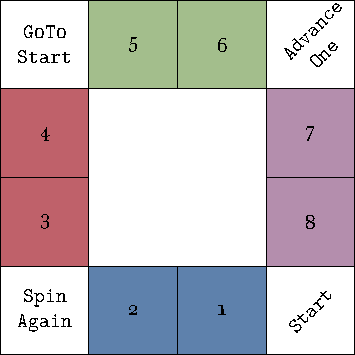
\includegraphics[width=.65\textwidth]{img/board.pdf}
	\caption{Board for the game described earlier.}
	\label{fig:miniopoly-board}
\end{figure}

First off, unlike the slot machine-playing robot, this robot 
player cannot entirely choose which square to move to, it can 
only decide if it wants to purchase it or not once it has 
landed on it. The biggest number it can spin is 4, and even if 
it got to spin again the furthest it could go is square 5. Even 
if the robot wanted to go to square number 8 and buy it, there 
is no possible way to do that.

Figure \ref{fig:miniopoly-diagram-start} shows a simplified 
version of the board. Only the squares accessible on the first 
turn are shown, along with arrows indicating the possible 
transitions between the starting square and the rest.
\begin{figure}[h]
	\centering
	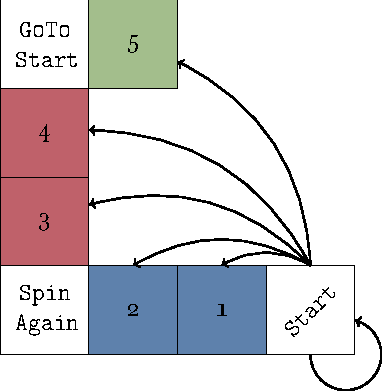
\includegraphics[width=.65\textwidth]{img/diagram-start.pdf}
	\caption{Squares accessible on the first turn.}
	\label{fig:miniopoly-diagram-start}
\end{figure}

In figure \ref{fig:miniopoly-diagram-start} we can see all the 
possible squares the robot might land on and then buy starting 
from the first turn. Notice how squares 6 and further are not 
included. If the robot were to spin a 4, the red square with 
number 3 is the furthest it could go. If it were to land on 
\texttt{Spin Again} and then spin a 4, the largest possible 
spin, it could move four squares: from \texttt{Spin Again} to 
3, then to 4, then to \texttt{Goto Start}, and finally to 
square 5, exhausting its possible moves.

Notice how in this figure we only care about the starting and 
ending points, not the transit points, so that is why there are 
no arrows pointing to the squares that move the player 
elsewhere like \texttt{Spin Again} and \texttt{Goto Start}. 
This is the reason there is an arrow that points from 
\texttt{Start} to itself. This transition might happen. In 
fact, we know what it takes for this to happen: land on 
\texttt{Spin Again}, and then land on \texttt{Goto Start}. In 
other words, this transition happens if the robot spins a 3 two 
consecutive times.

If the robot were to land on \texttt{Spin Again}, then spin a 
3, it would ``land'' on \texttt{Goto Start}, finishing its turn 
back at the starting square. That particular move results in 
the robot going back to the start and getting paid for 
completing the circuit, without running the risk of landing on 
a square someone else owns. That sounds like a very desirable 
move (for us looking at the big picture, the robot cannot see 
that far ahead yet). Since we would like this to happen, we 
might ask how likely is for that to happen.

\begin{figure}[h]
	\centering
	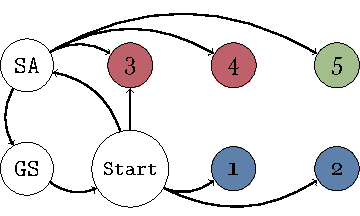
\includegraphics[width=\textwidth]{img/transicion.pdf}
	\caption{Diagram showing the possible transitions to the 
	numbered squares, starting the turn at \texttt{Start}. 
	Squares \texttt{GoTo Start} and \texttt{Spin Again} are 
	abbreviated as \texttt{GS} and \texttt{SA} respectively.}
	\label{fig:miniopoly-transicion}
\end{figure}

Lets try to analyze how likely the robot is to end up in this 
particularly rewarding situation. For that it's often helpful 
to think of the possible steps that lead to it. On figure 
\ref{fig:miniopoly-transicion} we can see a more abstract 
diagram of the possible movements the robot might make, and 
this time we are taking into account intermediate squares. Each 
arrow represents where the robot might land after spinning, not 
necessarily it's final resting square. Now, using some very 
basic probability theory we can calculate how likely it is for 
the robot to ``take that route'' so to speak. Once we do, we 
can calculate how likely a ``route'' or sequence of arrows is.

\begin{figure}[h]
	\centering
	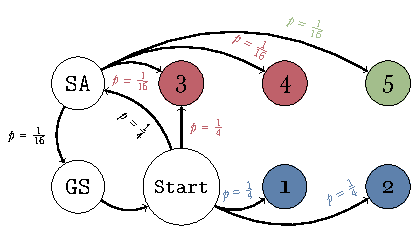
\includegraphics[width=\textwidth]{img/transicion-markov.pdf}
	\caption{Transition diagram with transition probabilities}
	\label{fig:miniopoly-transicion-markov}
\end{figure}

At the moment it is not important why some arrows have certain 
probabilities, and some might not be terribly obvious even for 
someone acquainted with some basic probability. In figure 
\ref{fig:miniopoly-transicion-markov} to find the probability 
of getting to a certain square (say 6 for example) we look only 
at the last arrow, as it takes into account the probability of 
the previous step happening. For example, the probability of 
the move that takes the player from \texttt{Start} back to 
\texttt{Start} we can look at the bottom left corner of figure 
\ref{fig:miniopoly-transicion-markov}. The player moves to 
\texttt{Spin Again} with probability 1/4 because the spinner 
has an equal chance of making the player move either 1, 2, 3 or 
4 squares. Once the player is on \texttt{Spin Again} and spins 
once more, it has a chance of 1/16 of landing on \texttt{GoTo 
Start}. The final arrow pointing from \texttt{GoTo Start} to 
\texttt{Start} is not annotated with the probability of it 
happening, since that transition is not random. Once the player 
lands there, the next thing that happens to the player is 
always the same: go to the starting square.

The robot we are trying to teach moves as the figure above 
suggests. There is a different diagram for each square in which 
the player finds itself at the start of its turn. The robot is 
not aware of this, all it knows is that it spins, and then is 
transported elsewhere and must decide whether to buy or not (if 
the square is available). All it knows is it's current 
position, and the gains or losses it sustained on the other 
squares it has visited. Crucially, landing on a square 
previously visited does not necessarily mean the reward will be 
the same as last time. For instance, if it lands on square 3 
and decides not to buy it, the reward was a net 0, but the 
other player may buy it so that the next time the robot visits 
that square it has to pay rent, which would mean a loss. Also, 
the reward for buying a square may come much later on or not at 
all. This robot must somehow keep track of what the expected 
reward for landing somewhere might be, recording it somewhere 
and tallying up as it goes.

For instance after a few turns it might have something fig. 
\ref{fig:hist-miniopoly} on its head to help make decisions.

After playing a few games, keeping a record of which squares it 
bought, the player might make a graph to discover what moves it 
made that resulted in higher rewards at the end of the game. 
Such a graph might look like figure \ref{fig:hist-miniopoly}, 
which is a violin plot. In this plot, a violin-shaped figure 
gives the robot an idea of what squares yielded better rewards 
or smaller losses when bought or when left for other players to 
buy. The height of the violin indicates how high the reward was 
at the end of the game, while the width of the violin helps the 
robot decide whether that outcome was a fluke or not. A thin 
violin at a specific height (reward) indicates that over the 
games it has played so far, that specific reward marked by the 
y-axis is not as common as the reward that corresponds to the 
thicker parts of the violin.
% Se entiende??

\begin{figure}
\centering
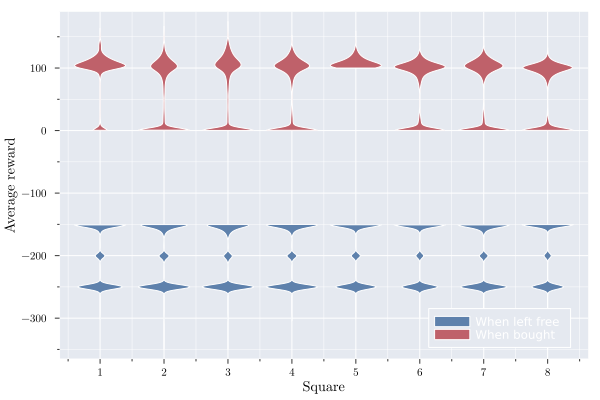
\includegraphics[width=\textwidth]{img/hist-miniopoly.tikz}
\label{fig:hist-miniopoly}
\caption{Violinplot}
\end{figure}

This figure was created by simulating N-THOUSAND games and 
recording what rewards the robot player obtained at the end of 
the game by buying or not buying a certain square. For 
instance, if it bought square 3, the record shows the initial 
loss of however much money the player paid for the square. 
Later on in the game if the opponent lands on square 3 and pays 
rent, that rent is recorded as a gain for the robot player. 
That number is averaged out at the end of the game so the robot 
can analyze this information later. One way of analyzing this 
information to improve strategy is precisely to make a graph 
like the one in figure \ref{fig:hist-miniopoly}

Its stands to reason that as this graph is updated the learning 
agent will be able to make progressively better choices by 
identifying the patterns. For instance, it might notice from 
figure \ref{fig:hist-miniopoly} that buying SQUARE ALGO 
consistently results in higher rewards at the end of the game. 
The robot noticed this because the violin corresponding to 
SQUARE ALGO is noticeably higher than the others. Simple as 
this example might be, the essence is similar to the powerful 
programs that defeat world champions of chess and Go.

This example covers most of the core ideas of what is referred 
to as the Reinforcement Learning Problem. We will explore the 
ideas presented here in much more detail along this thesis and 
crucially, focus on something we left out on this example. How 
can a purchase strategy be improved upon?

\section{Wrapping up}
So far we have developed a mental model of what to do should we 
wish to teach a robot how to drive or beat a world champion of 
Go. The rest of this thesis is dedicated to the careful 
development of the ideas here presented into the language of 
mathematics. Specifically, tackling questions such as:
\begin{itemize}
	\item What mechanism allows the robot player to learn from 
	experience and fine-tune it's strategy to become better?
	\item How can we tell when a new strategy is better than an 
	old one?
	\item Is it possible to find \textit{the} best strategy? 
	How difficult is it?
\end{itemize}

Beyond mere description, this exercise has the potential to 
unlock \textit{insight}. As is often said by legendary math 
communicator Grant Sanderson\footnote{From the YouTube channel 
\href{https://www.youtube.com/channel/UCYO_jab_esuFRV4b17AJtAw}{3blue1brown}}(loose 
quote), the point in formulating things this way is to gain a 
deeper understanding of the phenomenon. So let's dive right in.

	% \chapter{Optimization Theory}
\label{chapter:OptimizationTheory}

As teased in the previous chapter, the Reinforcement Learning Problem
is primarily a problem in optimization. The entire framing of finding
increasingly better ways to navigate the problem described is based on the theory
of mathematical optimization. This chapter aims to provide a suitable framing
for the remaining chapters, spinning a narrative thread that connects all the
problems to come. We focus less on specific results and more on their meaning
and geometric interpretation.

\section{Optimization as a geometric problem}

In the broadest possible terms, optimization problems are search problems. Such
search problems are often embedded in a geometric context.

\begin{wrapfigure}{I}{0.5\textwidth}
   \centering
   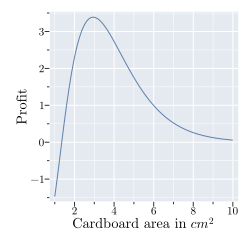
\includegraphics[width=0.5\textwidth]{img/1d-profits.tikz} 
   \caption{Profits function for the box-making company.}
   \label{fig:1d-profits}
\end{wrapfigure}

For an introductory problem, picture a company designing boxes. They have
conducted a study and isolated a relationship that describes their profits as a
function of the area of cardboard needed to make their boxes. This was initially
suspected, since the area of cardboard used to make the box determines the
volume.  Because of the company's pricing schemes, boxes with a certain volume
are more profitable than others. Recently, a relationship was confirmed as a
result of some analysis, a plot can be found in figure \ref{fig:1d-profits}. As
a result of the analysis, the relationship between cardboard area to make a box
and the company's profits was established to be a function $f: \R \to \R$. This
function takes as its only argument a real value that corresponds to the area of
cardboard used to make boxes, and returns a profit value. This company wants to
maximize profit by modifying the variable they can control: the area of
cardboard, and indirectly the volume of the box.

Picture for a moment that the graph shown in figure \ref{fig:1d-profits} is
unknown to the company (optimizing agent or simply agent henceforth), as
graphical representations are often not possible even if the exact nature of a
relationship is known. For instance, if the profits dependended on more than two
variables, a truthful graphical representation would not be available. By
plotting the profit function obtained from the analysis, finding the point that
maximizes profit is very straightforward. But since the optimizing agent may not
have this luxury, the agent must come up with a different strategy. The agent
then recalls that derivatives have a very useful geometric interpretation, they
give the slope of a function at a point. The agent can start by guessing a value
for the area of cardboard, and then find the point where the derivative equals
zero. Given that we have an explicit profit function we can calculate this
derivative, even if a graphical representation can not be given. The logic
behind the search for a zero is simple: if a function is continuous, has a
unique peak, and ``goes up'' on a certain subset of numbers, and then ``goes
down'' for the numbers right next, a peak is necessarily in between those two
regions. That peak corresponds to the point where the derivative equals zero.

\begin{wrapfigure}{I}{0.5\textwidth}
   \centering
   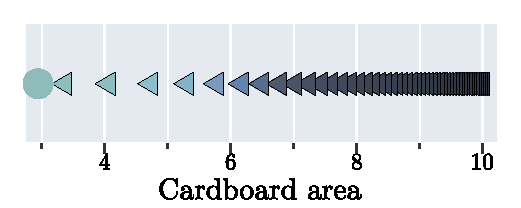
\includegraphics[width=0.5\textwidth]{img/gd-points.pdf} 
   \caption{Points the learning agent tried.}
   \label{fig:gd-points}
\end{wrapfigure}

With this in mind, the agent devises an ``educated guess'' algorithm to find the
point where the derivative equals zero, which is exactly where the peak of the
profits function is, as exemplified in figure \ref{fig:1d-profits}. The guessing
starts at the point where cardboard area equals 10. The agent evaluates the
derivative there, and finds that it is less than zero. In other words, the
profits would diminish if it were to try to use more than 10 square cm of
cardboard. So, the agent explores another point that is a fraction $\alpha$
smaller than the original guess. The agent continues this process changing the
value $\alpha$ as it goes. Figure \ref{fig:gd-points} shows the points this
agent tried while trying to achieve a maximum. The color of the point gets
lighter as it approaches the maximum, as color represents the value of the
profit function at the point. The colors get lighter as profit increases. The
markers show the direction in where the next exploration point will be, the
stopping point is marked by the circle.

Most computational methods for optimization rely on the same basic ideas as our
``educated guess'' algorithm. Since exact solutions are too computationally
expensive to calculate, or even impossible in some instances, optimization
algorithms take starting points in the seach space where an optimal point would
be found and explore that space iteratively by means of some mechanism where
almost each new iteration is closer to an optimal point than the previous one.
In the case of the algorithm described so far, the mechanism to approach
optimality is based on the observation that peaks correspond to zeros of the
derivative of the function being optimized (objective function).

The algorithm we have been calling ``educated guess'' is in fact known as the
gradient descent. A ``gradient'' is the generalization of the concept of a
derivative for functions of the form $f: \R^{n} \to \R$. Let us define gradient
descent by defining an operator $D$ that acts on points in $\R^{n}$. We choose
to present the algorithm in terms of operators as it makes some crucial ideas in
chapter \ref{chapter:ApproximateLinearP} more palletable.

\begin{dfn}{Gradient Descent Operator}{}
    We define the \emph{gradient descent} operator, denoted by $D: \R^{n} \to
    \R^{n}$ for a given function $f: \R^{n} \to \R$ as
    \[
        D \vec{x} = \vec{x} - \alpha \nabla f(\vec{x}), \quad \alpha > 0.
    \]
\end{dfn}

By using the Gradient Descent Operator, we can define a sequence
$\{\vec{a}_n\}$ of points in $\R^{n}$. The sequence is defined as
$\vec{a}_{n+1} = \vec{a}_n - \alpha_n \nabla f(\vec{a}_n)$. By thinking of the
process in terms of operators, finding optimal points (as they may not be
unique) is simply finding points $a_*$ that satisfy
\[
    D a_* = a_*.
\]
When some $a_*$ satisfies the condition above, we say that $a_*$ is a
\emph{fixed-point} of operator the $D$. In other words, the optimization problem
the box-making company faces can be reduced to looking for fixed points of
operator $D$ in some geometric space. It can be proved that such a fixed point
exists whenever $f$ satisfies a certain set of conditions, but reviewing them
now would be beside the point. We review the conditions and leverage them to
guarantee the existance of optimal solutions to the Reinforcement Learning
Problem in chapter \ref{chapter:ApproximateLinearP}.

The problem just presented has several characteristics that make gradient
descent a good approach to solving it. Some other characteristics that define
the problems for which gradient descent is well suited are:
\begin{itemize}
    \item The objective function $f$ must be differentiable and remain the same
        throughout the process.
    \item The space being searched for optimal solutions is free of any
        restrictions.
    \item The exploration process has no effect on the optimal solution to be
        found. In contrast, some problems have different, branching possibilities.
        In the case described here, if an optimal solution exists it is fixed and
        cannot be altered.
\end{itemize}
The Reinforcement Learning Problem presented earlier is an example of a problem
that can not be solved using the same techniques used in the last example. One
of the main reasons why, is the fact that the \ac{rl} problem involves
sequential decision making. Making a decision at some point can change the
outcome of the process drastically. For instance, when playing chess, some moves
are so crucial that may determine the outcome of the game.

\section{Working with constraints}

After using gradient descent to maximize their profits, the box-making company
wants to include more factors into their analysis to replicate their success at
making their operation more efficient. They have noticed that their profits,
apart from being dependent on the amount of cardboard needed to make their
best-selling box, depend on the number of envelopes they make. The company has
some knowledge that has to be incorporated into the search for profit
maximization:
\begin{itemize}
    \item Each envelope produced uses 100 square centimeters of cardboard.
    \item Month to month they can only buy 10,000 square centimeters of cardboard.
    \item The biggest boxes they can make use 10 square meters of cardboard.
    \item The machine can produce a maximum of 10,000 envelopes per month.
\end{itemize}


\begin{wrapfigure}{I}{0.5\textwidth}
   \centering
   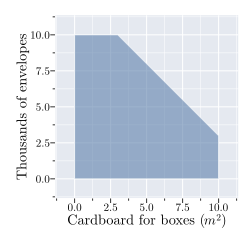
\includegraphics[width=0.5\textwidth]{img/feasible-region.tikz} 
   \caption{Combinations of box volume and number of envelopes the company can produce.}
   \label{fig:feasible-region}
\end{wrapfigure}

The search space the company has to explore now is not like the one in the
previous example. We are only interested in combinations of box volume and
cardboard amount that satisfy the conditions laid out by the company. In figure
\ref{fig:feasible-region} the optimizing agent (the company) plotted all the
possible combinations of the amount of cardboard they can use for their boxes,
and the number of envelopes they will produce. Points inside the blue area
satisfy the conditions, while points outside do not. The region in blue is
called the \emph{feasible region} for this problem. The solution must lie inside
the feasible region, we are not interested in looking outside.

When the profit function can be expressed as multiples of cardboard area for
boxes plus number of envelopes this optimization problem is called a
\emph{linear program}. In practice linear programs have desirable properties,
such as: the existence and location of their solutions, and the affordable
amount of computational power they need to be solved. The classic algorithm
called \emph{simplex} uses clever geometric manimpulations to explore the
corners of the feasible region efficiently. The main results reviewed in this
thesis establish that a Reinforcement Learning Problem like the Miniopoly
example in chapter \ref{chapter:Motivation} can be cast as a linear program. The
rest of this thesis deals with the specifics like
\begin{itemize}
    \item How to choose an objective function?
    \item What characterizes optimal solutions?
\end{itemize}
	% In Chapter \ref{chapter:Motivation}, we briefly reviewed the areas that
constitute the field of Machine Learning and motivated an introductory example
to Reinforcement Learning. We highlighted the differences between Supervised
Machine Learning (supervised ML) and RL by contrasting the way each work.
Supervised ML receives a wealth of examples from which it must extract patterns,
while RL receives no input data and so has to learn by interacting with its
environment. Supervised ML is often tasked with classifying or predicting a
response. In this thesis, we focus only on the classification task.

\section{Classification}
Supervised ML algorithms tasked with classifying receive large amounts of
labeled data. Through the process called ``fitting'' or ``learning'', the
algorithm will (hopefully) label correctly new observations never seen before.
The classification task seeks to find a systematic way of predicting a
phenomenon given a set of measurements.

\subsection{Formalizing}
Putting some concepts to work, picture a scenario where we have access to
several measurements (e.g., age, weight, blood pressure, etc\dots) for a group
of patients. Some patients in the study group suffered a stroke; the rest did
not. Our task is to find a systematic way of predicting whether or not a new
patient not studied before will suffer from a stroke by measuring the same
variables measured for the initial group.

Fundamentally, a supervised ML algorithm must receive a \textit{training set}, a
set of pre-labeled data from a knowledgeable source, in contrast with RL, where
labeling is often not even possible or practical. This source of truth, the
training set, is a set of observations $(\vec{x}_1, y_1), \dots, (\vec{x}_n,
y_n)$. The vectors $\vec{x}_i = [x_1, x_2, \dots, x_p]^{\top} \in \R^{p}$ can be
thought of as a list of measurements of every variable of interest for the
$i$-th observation. In the case of the example trying to predict strokes, $x_1$
would correspond to age, $x_2$ to weight, and so on. The training set also
contains $y_1, \dots, y_n$, one-dimensional values we call variables or labels
in the specific case of classification. Using the standard parlance, following
\cite{louppe2014}, the input variables are known as \textit{features}, input
vectors as \textit{instances} or \textit{samples} and the output variable as
\textit{target}. For our purposes, we consider that the target variable is
always categoric, not numeric or continuous. Nevertheless, continuous target
variables are allowed, but the learning task is called regression, which is
outside this thesis's scope.

In a typical ML workflow, the algorithm used to make predictions is trained on
the set we just described. Its performance is tested on a different set of
similar data that the algorithm had no access to during its training period.
From now on, we denote the training set as $\L$. For convenience we group the
feature vectors into a \textit{feature matrix} $X \in \R^{p \times n}$, where
the $i$-th column is $\vec{x}_i$. Similarly, we group the target variables into
the vector $\vec{y} \in \R^{n}$.

Our classification task can be framed as finding a function $f_{\L}$ we will
call model whose output or predictions $f_{\L} (\vec{x}) = \widehat{\vec{y}}$
are ``as good as possible''. We subscript the function $f$ with $\L$ to
highlight that the function depends on what data the learning set contains. We
proceed to define what makes a model ``good'' at making predictions.

\subsection{Evaluation}
As it has become a recurring theme in this thesis, determining what makes a
prediction suitable and finding the best possible model $f_\L$ is a process of
optimization. Since we assume that the learning set is a sample of the
population we aim to label with our model, it stands to reason that a model that
makes the fewest mistakes when tasked with classifying the training observations
will also make the fewest mistakes when classifying new observations. In
reality, that is not precisely the case, as often making the number of
classification mistakes as small as possible in the training set results in a
model that ``memorized'' the set and has no ability whatsoever to generalize
patterns. It only reproduces known-good answers. But the idea is not entirely
misguided, it provides a good starting point.

The process we referred to as ``fitting'' a model consists of finding a model
which minimizes its expected prediction error.

\begin{dfn}{Prediction or Generalization Error}{generalization-error}
    The expected \emph{prediction} or \emph{generalization} error of a model
    $f_\L$ is the probability of misclassification of the model
    \begin{equation*}
        \Err (f_\L) = \mathbb{E} \left[ \1 (y_i \neq \widehat{y}_i)  \right].
    \end{equation*}
    Where $\widehat{y}_i \coloneqq f_\L (\vec{x}_i)$ is the model's prediction
    for the observation $\vec{x}_i$, and the indicator function $\1$ equals one
    whenever the condition inside it holds, and zero otherwise.
\end{dfn}

Minimizing this Generalization Error will allow us to classify the newest
observations committing as the lowest possible number of errors overall.
Including observations never seen before, not only the ones we have access to in
the training set. Since the distributions for observations $(\vec{x}_j, y_j)$
are generally not known, we must estimate the generalization error. Several
techniques to solve this problem exist but are numerous and outside of scope.
From now on, we denote as $\widehat{\Err}$ an estimator of the generalization
error.

The term ``fitting'' when discussing finding a suitable model is a consequence
of how such a model is found. Since the generalization error is not directly
measurable and thus not directly minimizable, we have to use a reasonable
approximation. We assume that a family of candidate models, $\mathcal{H}$ known
as hypotheses, exists. Our optimization target then becomes to find the best
model among the space of hypotheses. To be more specific, let $\vec{\theta}$ be
the vector of hyper-parameters controlling the behavior of a specific model.
Then, our optimization task is to find $\theta^{*}$,
\begin{equation*}
    \theta^{*} \coloneqq \argmin_{\theta} \widehat{\Err}(f_\L (\vec{x}; \theta)) \quad \forall \vec{x}.
\end{equation*}

Many classification models are available, each leveraging different
properties and resulting in different strengths and weaknesses. The optimization
problem involved in fitting each one is different from the rest. For this thesis, we focus on one specific model: classification trees. We
introduce them here and show in part II how fitting them gives way to an
optimization process analogous to a Reinforcement Learning problem and frame it
as such so we can leverage the power of RL to fit classification trees.

\section{Classification Trees}
Classification trees and, more generally, classification and regression trees
are Machine Learning models like the ones described in the previous section.
They have gained massive popularity in the recent and ongoing boom in machine
learning for their numerous qualities. For instance, they can model arbitrarily
complex relationships in data, handle both numeric and categorical data, and are
easily interpretable as they result in simple decision rules. Most importantly,
they are the building block of state-of-the-art algorithms for ML, such as
XGBoost \cite{XGBoost}.

Sadly, their fitting process leads to a rather complicated problem that cannot
be solved exactly in a reasonable time. The fitting process shares many
similarities with the RL problem, which is described in a wealth of detail in
Chapter \ref{chapter:ReinforcementLearning}. This similarity is the foundational
idea of this thesis, and we hope to show in part II how an alternative
methodology to fitting trees can be developed by leveraging the techniques used
in RL. With that goal in mind, it is time to lay the foundations behind trees'
structure.

\subsection{Tree models}
Let $\Omega = \left\{ (\vec{x}_i, y_i) \right\}$ be the space of all possible
feature-target pairs. When each feature $y$ is part of a set of categories
$\mathcal{C} \coloneqq \left\{ c_1, c_2, \dots, c_j \right\}$, another way to
look at the classification task is to define a partition over $\Omega$ taking
advantage of the natural distinction our set of categories provides.
\begin{equation*}
    \Omega = \bigcup_{i=1}^{j} \Omega_{c_i},
\end{equation*}
where each $\Omega_{c_i}$ is defined as $\left\{ (\vec{x}_k, y_k) \mid y_k = c_k
\right\}$.

Similarly, a model $f_\L$ defines a partition. This partition however is made
over the input space $\mathcal{X} = \left\{ \vec{x}_i \mid (\vec{x}_i, y_i) \in
\Omega \right\}$. This partition can be described as the preimages of $f_\L$ as
such
\begin{equation*}
    \mathcal{X} = \bigcup_{i=1}^{j} f_{\L}^{-1}(\Omega_{c_i}).
\end{equation*}
The classification task then can be thought of as learning the model $f_\L$ that
gives the partition of $\mathcal{X}$ that most closely approximates the
partition on $\Omega$ as a result of its preimages.

In other words, we are trying to represent $f$ as a tree (in the same way
Computer Science thinks about trees) where any node $t$ represents a subspace
$\mathcal{X}_t \subseteq \mathcal{X}$ of the input space such that the node
designated as root (denoted $t_0$) corresponds to the entirety of $\mathcal{X}$.
Internal nodes $t$ are originated via a \textit{split} $s_t$ taken from a set of
question $\mathcal{Q}$.

The set of questions $\mathcal{Q}$ is exactly what it sounds like. The question
defining split $s_t$ might be, for example, is $x_m < 65$? Or, is the person
recorded as observation $m$ younger than 65? The space $\mathcal{X}_t$
represented by node $t$ is made up of disjoint subspaces corresponding to each
of $t$'s children nodes; two in the case of binary trees. 

Terminal nodes (or leaves) are labeled with a best guess value $\widehat{y}_t
\in \mathcal{C}$. The prediction process is carried out by navigating the tree,
providing answers to the questions defining each node until a leaf is reached.
The label for that leaf will be the tree's prediction. In algorithm
\ref{alg:tree-predict}, we show a formal description of the process.

\begin{algorithm}
    \SetKwFunction{Predict}{predict}
    \KwIn{The tree $f_\L$}
    \KwIn{The feature vector $\vec{x}$}
    \KwOut{The predicted class $\widehat{y}$ for $\vec{x}$}
    \Function{\Predict{$f_\L, \vec{x}$}}{
        $t \gets t_0$ \;
        \While{$t$ is not a terminal node}{
            $t \gets$ the child node $t'$ of $t$ such that $\vec{x} \in \mathcal{X}_t$ \;
        }
        \Return{$\widehat{y}_t$} \;
    }
    \caption{Predict output value $\widehat{y}$ with tree $f_\L$
        \cite[Ch.~3.2]{louppe2014}.}
    \label{alg:tree-predict}
\end{algorithm}

[Maybe una imágen de muestra de el árbol particionando el espacio.]

\subsection{Fitting Decision Trees}
\citeauthor{hyafil1976} proved that fitting a decision tree that minimizes the
generalization error is an NP-complete problem \cite{hyafil1976}. That means no
polynomial time algorithm to solve it exists. As with other NP-complete
problems, the solution methods must rely on heuristics. One of the most widely
used algorithms for tree fitting is the CART (Classification and Regression
Tree) algorithm developed by \citeauthor{breiman2017} \cite{breiman2017}; it is
implemented in scikit-learn\footnote{The industry-standard python library for
machine learning \cite{louppe2014}.}, available to R users via the tidymodels
extension and part of MLJ.jl\footnote{The most widely used machine learning
library for Julia users.}. This thesis will focus on CART and later on try to
extend it.

The CART algorithm is based on greedily finding splits based on node purity, the
amount of misclassified observations in a given node. The \textit{purer} the
node, the lower the impurity score, the better the prediction. We denote by
$\L_t$
\begin{equation*}
    \L_t \coloneqq \left\{ (\vec{x}, y) \mid \vec{x} \in \mathcal{X}_t \right\}.
\end{equation*}
Many impurity functions can be used to determine the goodness of a split, each
with their benefits and drawbacks. We only discuss the impurity decrease at the
moment, since it is not necessary to have a specific impurity function to
describe the fitting algorithm nor do we have enough space to cover the
available options and their properties.

\begin{dfn}{Impurity decrease}{}
    The \emph{impurity decrease} of a binary split splitting node $t$ into a
    left child $t_L$ and a right child $t_R$ is
    \begin{equation*}
        \Delta i(s, t) \coloneqq i(t) - \frac{N_{t_L}}{|\L_t|} \, i(t_L) - \frac{N_{t_R}}{|\L_t|} \, i(t_R),
    \end{equation*}
    where $N_{t_L}$ and $N_{t_R}$ are the number of observations contained by
    nodes $t_L$ and $t_R$ respectively.
\end{dfn}

It is straightforward to see the similarity of the impurity decrease definition
with how an expected value is estimated since $N_{t_L} / |\L_t|$ is the
probability of a given observation falling to the left node. In simple words,
the impurity decrease for node $t$ is simply the original impurity minus the
expected value of the impurity of its children. Keeping in mind that the
proportion $N_{t_L} / |\L_t|$ represents the probability of a given observation
being in the left child of $t$, we refer to it as $p_L$; denoting $p_R$ the
analog for the right child.

We have the tools to define a formal procedure for greedily fitting a binary
classification tree in algorithm \ref{alg:tree-fit}. The pseudocode presented
here lacks a litany of essential considerations, such as stopping criteria,
splitting rules, and impurity functions. We are limited to presenting a broad
picture, as exploring even some of the deficiencies mentioned would require
entire books.

\begin{algorithm}
    \SetKwFunction{Fit}{fit}
    \SetKwFunction{Pop}{pop}
    \SetKwFunction{Push}{push}
    \KwIn{The training set $\L$}
    \KwOut{A fitted binary classification tree $f_\L$}
    \Function{\Fit{$f_\L$}}{
        Create an empty tree $f_\L$ with root node $t_0$ \;
        Create an empty stack $S$ of \emph{open} nodes $(t, \L_t)$ \;
        Append $(t_0, \L)$ to $S$ \;
        \While{$S$ is not empty}{
            $t, \, \L_t \gets S$.\Pop{} \;
            \If{stopping criteria are not met}{
                $\widehat{y}_{t} \gets$ some constant value \;
            }\Else{
                Find the split $s_*$ on $\L_t$ that maximizes impurity decrease
                \[
                    s_* = \argmax_{s \in \mathcal{Q}} \Delta i(s, t)
                \]
                \;
                Partition $\L_t$ into $\L_{t_L}$ and $\L_{t_R}$ according to $s_*$ \;
                Create the left and right children nodes $t_L, t_R$ of t \;
                $S.$\Push{($t_R, \L_{t_R}$)} \;
                $S.$\Push{($t_L, \L_{t_L}$)} \;
            }
        }
        \Return{$f_\L$} \;
    }
    \caption{Greedy fit of a binary classification tree
        \cite[Ch.~3.3]{louppe2014}.}
    \label{alg:tree-fit}
\end{algorithm}

Splitting rules will be crucial for developing the rest of this thesis, so we
must discuss them, even if only briefly. The true magic of the algorithm lies in
the splitting strategies and the termination criteria.

\subsection{Splitting rules}

\begin{dfn}{Split}{split}
    A \emph{split} $s$ of node $t$ is a partition of $\mathcal{X}_t$. Formally, a partition is a collection of non-empty subsets of $\mathcal{X}_t$ such that,
    \begin{enumerate}
        \item The union of every subset equals $\mathcal{X}_t$
        \item The intersection of any two distinct subsets is empty.
    \end{enumerate}
\end{dfn}

The number of possible partitions of $\L_t$ into $k$ non-empty subsets is given
by the Stirling number of the second kind \cite{louppe2014}
\begin{equation*}
    S(N_t, k) \coloneqq \frac{1}{k!} \sum_{j=0}^{k} (-1)^{k-j} \binom{k}{j} j^{N_t}.
\end{equation*}
Even in the case of binary partitions in which $s(N_t, k)$ reduces to $2^{N_t
-1}-1$, the number of partitions grows exponentially and, even worse,
factorially for the non-binary case. Calculating each possible partition and
choosing the best is not computationally feasible. The attentive reader will
find the similarities when describing in full detail the RL problem presented in
Chapter \ref{chapter:ReinforcementLearning}. The best binary split $s_*$ can be
found using algorithm \ref{alg:best-binary-split}.

\begin{algorithm}
    \SetKwFunction{BestSplit}{FindBestSplit}
    \KwIn{A subset $\L_t$ of the training set $\L$}
    \KwOut{The best binary split $s_*$ on $\L_t$}
    \Function{\BestSplit{$\L_t$}}{
        $\Delta \gets - \infty$ \;
        \For{$j \gets 1, \dots, p$}{
            Find the best binary split $s_{*}^{j}$ for the variable $X_j$ \;
            \If{$\Delta i(s_{*}^{j}, t) > \Delta$}{
                $\Delta \gets \Delta i(s_{*}^{j}, t)$ \;
                $s_* \gets s_{*}^{j}$ \;
            }
        }
        \Return{$s_{*}$} \;
    }
    \caption{Find best binary split $s_*$ for node $t$ \cite[Ch.~3.6.3]{louppe2014}.}
    \label{alg:best-binary-split}
\end{algorithm}

It can be proved that the complexity of algorithm \ref{alg:best-binary-split} is
constrained by the complexity of the sort operation \cite[Ch.~5]{louppe2014}.

With algorithm \ref{alg:best-binary-split}, we have enough background to examine
the similarities between the problem that arises from fitting a classification
tree and the more general reinforcement learning problem in part II.

\section{Bibliographical notes}
As mentioned, we had to skip several details necessary for an actual
implementation of the tree-fitting algorithm. They are not strictly mandatory
for the purposes of this thesis but are vastly interesting and worthwhile in
their own right. To clarify or expand upon the concepts presented here, please
refer to the sources used to develop this chapter:
\begin{enumerate}
    \item \citeauthor{breiman2017}'s book \citetitle{breiman2017}. One of the
        cornerstone texts for this subject and the first formal descriptions of
        the CART algorithm \cite{breiman2017}.
    \item The standard textbook for modern machine learning algorithms and
        applications: \citetitle{elements2009}. This source is particularly good
        for reviewing the foundations of statistical, supervised learning in
        much more depth and in a better style that could be achieved here
        \cite{elements2009}.
    \item \citeauthor{louppe2014}'s doctoral thesis, which is heavily cited in
        this chapter. Louppe is a core developer emeritus of the scikit-learn
        python library, the industry-standard library. His work is admirably
        deep, clear, and has valuable insights on the real-world considerations
        a practical implementation would have to keep in mind \cite{louppe2014}.
        After extensive research, this source provided the most satisfying
        treatment of classification and regression trees of all documents
        reviewed.
\end{enumerate}

The field of machine learning is so vast that we only had a chance to develop
the most rudimentary, essential ideas we will need. Reading the sources cited
for this chapter is encouraged.
	
\label{chapter:ReinforcementLearning}

On Chapter~\ref{chapter:motivation} we presented a very simple 
example of a problem that may be solved via Reinforcement 
Learning: a robot trying to play a game we called Miniopoly. As 
simple as that example was, the key ideas will now allow us to 
delve into the theory proper, and formalize some ideas while 
hopefully giving satisfying answers to some questions that the 
intuitive treatment might have left open.

\section{The Agent \& the Environment}
Recall from Chapter~\ref{chapter:Motivation} that we referred 
to the robot player as a ``learning agent''. This agent is 
continuously interacting with the rest of the game and 
surveying its current state. As we saw earlier, the robot then 
selects an action on the basis of this current game state.

To be precise, say that the game starts at some $t=0$ and ends 
at $t=T$. We discretize this period of time into $t \in \{0, 1, 
2, \ldots \}$ At each of these points $t$ in time, the agent 
finds itself at some state $S_t \in \States$, where $\States$ 
represents the set of all possible states. This defines exactly 
what we called a stochastic process back in 
Chapter~\ref{chapter:Stochastic}: a series of random variables 
$\{ S_t \}_{t = 0, 1 \ldots}$. 

Likewise, at each time step $t$ the agent chooses how to 
interact with an action $A_t \in \Actions(s)$, where 
$\Actions(s)$ is the set of all \textit{available} actions at 
the current state $s$. This too forms a stochastic process. One 
time step in the future $t+1$ the agent receives more feedback 
from the environment, the so-called reward signal $R_{t+1} \in 
\Rewards \subseteq \R$. This process moves forward from $t$ to 
$t+1$ and so on until the task is over. This defines a Markov 
Decision Process (MDP from now on), which we can reorder as 
follows:
\begin{equation}
	S_0, A_0, R_1, A_1, R_2, S_2, A_2, R_3, \ldots
\end{equation}

This particular ordering makes it easy to see why we chose to 
discretize time into steps. This illustrates how at each time 
step the agent surveys the state, and based on it selects a 
\textit{feasible} action. The next time step begins when the 
robot receives a reward signal from the environment. 

A key idea is subtly hidden in the notation. Notice how only 
the set of actions depends on a particular $s$. Both the set of 
states $\States$ and the set of rewards $\Rewards$ are in a 
certain sense independent of $s$. Why is it that only 
$\Actions(s)$ is dependent on $s$?

The ``Markov'' in Markov Decision Process is exactly what makes 
the set of actions special. As covered in 
Chapter~\ref{chapter:Stochastic}, a Markov process is often 
used to describe stochastic transitions between a set 
of---emphasis on terminology here---\textit{states}. In the 
example on Chapter~\ref{chapter:Motivation} the states were the 
literal squares in the game. And as we discussed, not every 
state is accessible from any other state. Thus, it makes sense 
that for each state the set of possible actions is determined 
by it. Some transitions are just impossible.

Not only are some transitions impossible at certain states, a 
given action chosen by the agent will not always result in the 
same transition from the state $s$ to the state $s'$, which 
might sound obvious as we have already established that this 
entire process can be best modeled by a MDP. To study the 
probability of a certain transition from state $s$ to state 
$s'$ given that a certain action $a \in \Actions(s)$ was taken 
we introduce the \textit{dynamics} function, keeping with the 
notation in \cite{SuttonBarto}.

\begin{dfn}{Dynamics function}{dynamics-func}
	For all $s, s' \in \States, r \in \Rewards, a \in 
	\Actions(s)$, we define the \emph{dynamics function} $f: 
	\States \times \Rewards \times \States \times \Actions(s) 
	\to [0, 1]$ as follows:
	\begin{equation*}
		p(s', r \mid s, a) \coloneqq \IP{S_t = s', R_t = r 
		\vertsep S_{t-1} = s, A_{t-1} = a}.
	\end{equation*}
\end{dfn}

Hola \ref{dfn:dynamics-func}


% FIXME: ESTO NO TIENE CONTEXTO, PONERLO
\begin{equation}
	\label{eq:prop-dependencia-vq}
	v_* (s) = \max_{a \in \Actions} q_* (s, a) \quad \forall \s in \States.
\end{equation}

\part{Approximate solutions to the Reinforcement Learning Problem}
\label{part:II}

	% \chapter{Approximate Linear Programming}
\label{chapter:ApproximateLinearP}
\section{Introduction}

As discussed in previous chapters \ref{chapter:ReinforcementLearning}, the
problem of finding the best policies by using Bellman's optimality equations
falls within the realm of dynamic programming. The problem is that even if an
explicit solution can be given under certain conditions, the computational
burden of calculating exact solutions is often too significant to overcome, even
on modern computing equipment. And given the ``curse of dimensionality'', even
if the contemporary problems became tractable in the future thanks to the
ever-increasing computing power, that very same improvement in computing power
would motivate researchers to tackle bigger still problems. So, to use the
\ac{rl} techniques, we must find a way to use our computational resources more
efficiently. 

Since Reinforcement Learning happens to be part of the techniques often grouped
under the umbrella of ``artificial intelligence'', it has enjoyed much attention
for decades. Thanks to these research efforts and numerous applications in the
industry, there are several battle-tested approximate solutions to the \ac{rl}
problem we have developed here. Among these are: Q-learning, Monte--Carlo
estimation methods, temporal difference learning, and many others that are
described in detail in \cite[Chapter~4]{SuttonBarto}. The somewhat novel
technique described in this thesis was developed in the first decade of the
2000s and is not part of the standard toolbox for solving \ac{rl} problems since
it was developed initially in the area of management science and particularly
for the problem of probabilistic inventory management, following previous work,
laid out since the 1960s. 

Specifically, the technique to be laid out in this part of the thesis was
developed by \citeauthor*{farias2003LP2ADP}, as a continuation of previous work
by \citeauthor*{denardo1970} and \citeauthor*{depenoux1963} in
\cite{denardo1970} and \cite{depenoux1963}, respectively. In a nutshell,
\citeauthor*{farias2002thesis} casts the dynamic programming problem that arises
from solving Bellman's optimality equations as a linear program and then gets
around the curse of dimensionality by using linear approximations for the
interest functions to reduce the number of variables in the problem. Without
further ado, let us get to the details right after developing the necessary
background.

\section{Exact Dynamic Programming}

In Chapter \ref{chapter:ReinforcementLearning}, we showed that using Bellman's
optimality equations, we can obtain optimal policies if we have access to the
optimal value ($v_*$) or action-value ($q_{*}$) functions. We denote these
functions subindexed by $*$ to accentuate the fact that they are optimal in the
sense that they satisfy Bellman's optimality equations, which are
\eqref{eq:bellmans-value} and \eqref{eq:bellmans-action-value} for $v_*$ and
$q_*$ respectively. 
\begin{align}
v_{*}(s) &= \max_{a} \sum_{s', r} p(s', r \mid s, a) \left[ r + \gamma v_{*} (s')
\right], \label{eq:bellmans-value} \\
q_{*}(s, a) &= \sum_{s', r} p(s', r \mid s, a) \left[ r + \gamma \max_{a'} q_{*}
(s', a') \right], \label{eq:bellmans-action-value}
\end{align}
for all $s \in \States, a \in \Actions$.

Equation \eqref{eq:bellmans-value} is important, but not that helpful in
practice. It tells us the best possible reward a learning agent can expect in a
learning task. In other words, the best possible reward \textit{after} the agent
followed the best policy but tells us very little about how to obtain that
policy. We would like to predict the total reward a given policy will yield.
Thankfully, in chapter \ref{chapter:ReinforcementLearning}, we obtained an
expression to calculate the expected reward a given policy $\pi$ will yield
starting from a certain state $s$, that we will refer to as \textit{Bellman's
recurrence equation} from now on: 
\begin{equation}
\label{eq:bellmans-recurrence}
% TODO: Transcribir (4.4) de S&B.
v_\pi (s) = \sum_{a \in \Actions} \pi(a \mid s) \sum_{s', r} p(s', r \mid s, a) \left[ r + \gamma v_{\pi}(s') \right].
\end{equation}

The identity \eqref{eq:bellmans-recurrence} was proved earlier in chapter
\ref{chapter:ReinforcementLearning} in Lemma \ref{lem:recursive-eval}, the
Recursive Evaluation Lemma. We named the Lemma that way for reasons that will
become apparent soon.

Using \eqref{eq:bellmans-recurrence} we can obtain an exact solution for $v_\pi$
solving one equation for each state $s \in \States$. This is often called the
\textit{prediction problem} in the literature \cite[Chapter~4.1]{SuttonBarto}.
Transforming equation \eqref{eq:bellmans-recurrence} we obtain the following,
simpler expression:
\begin{align}
\label{eq:bellmans-recurrence-prime}
v_\pi(s) &= \sum_{a} \pi(a \mid s) \sum_{s', r} p(s', r \mid s, a) \left[ r + \gamma v_\pi (s') \right] \nonumber \\
&= \sum_{a} \pi(a \mid s) \left[ \sum_{s', r} r p(s', r \mid s, a) + \gamma \sum_{s', r} v_\pi (s') p(s', r \mid s,a) \right] \nonumber \\
&= \sum_a \pi(a \mid s) \underbrace{\sum_{r} r \sum_{s'} p(s', r \mid s, a)}_{r(s,a) \text{(by dfn. \ref{dfn:rewards-func})}} +
    \gamma \sum_{a} \pi(a \mid s) \sum_{s', r} v_\pi (s') p(s', r \mid s, a) \nonumber \\
&= \sum_{a} \pi(a \mid s) \left[ r(s,a) + \gamma \sum_{s'} p(s' \mid s, a) v_\pi (s') \right] \tag{\ref*{eq:bellmans-recurrence}$\prime$}.
\end{align}

Since \eqref{eq:bellmans-recurrence-prime} defines one equation for each state,
we can think of the system of linear equations defined in terms of vectors and
matrices. This approach will later serve to define Bellman's policy\footnote{or
``one-step'' \cite[pg.~9]{nadeemward2021}, or ``expectation backup''
\cite[Lect.~3, Contraction Mapping]{silver2015}, the literature uses various
names. We follow \cite{raoRL4F}.} and optimality operators, a powerful tool.

For now, let us consider the value function as a vector, following
\cite[pg.~132]{raoRL4F}. Specifically,
\[
    \vec{v} = \left[ v (s_1), \dots , v (s_{|\States|}) \right].
\]
As shorthand notation we define $\vec{v}(s) \coloneqq v(s)$. Recall that $r(s,
a)$ is the expected reward upon taking action $a$ being in state $s$, and $p(s'
\mid s, a)$ is the probability of transitioning directly from state $s$ to state
$s'$ after taking action $a$. We define:
\begin{align*}
    R_\pi (s) &= \sum_{a \in \Actions} \pi(a \mid s) \, r(s,a), \\
    P_\pi (s, s') &= \sum_{a \in \Actions} \pi(a \mid s) \sum_{s' \in \States} p(s' \mid s, a),
\end{align*}
which result from a slightly rearranged version of
\eqref{eq:bellmans-recurrence-prime}.

We denote by $\vec{R}_\pi$ the vector $\left[ R_\pi(s_1), \dots, R_\pi
(s_{|\States|}) \right]$ and $\vec{P}_\pi$ the stochastic matrix $\left[
P_\pi(s_i, s_j) \right]$ that defines the transition probabilities from any
state $s_i$ to every other distinct state $s_j$ with $i, j \in \left\{ 1, \dots,
|\States| \right\}$. As promised, this is the key to what will become one of our
most powerful tools: Bellman's policy operator.  This will enable us to study
how \textit{any} $v$ acts on the set of states $\States$.

\begin{dfn}{Bellman's Policy Operator}{bellmans-pol-operator}
    We denote by $T_\pi$ the operator $T_\pi: \R^{|\States|} \to \R^{|\States|}$
    defined as:
    \[
        T_\pi \vec{v} = \vec{R}_\pi + \gamma \vec{P}_\pi \vec{v},
    \]
    for any value function vector $\vec{v} \in \R^{|\States|}$. The definition
    of this operator can be found in \cite[Ch.~5.4]{raoRL4F}.
\end{dfn}

Using the newly defined Bellman's Policy Operator, we can rewrite Bellman's
recurrence equation \eqref{eq:bellmans-recurrence} as
\begin{equation}
    \label{eq:BPO-fixed-point}
    T_\pi \vec{v}_\pi = \vec{v}_\pi.
\end{equation}
This means $\vec{v}_\pi$ is a fixed point of the Bellman Policy Operator.

Using the same arguments that led to \eqref{eq:bellmans-recurrence-prime}, let
us write Bellman's optimality equation for the value function
\eqref{eq:bellmans-value} using another operator.

\begin{dfn}{Bellman's Optimality Operator}{bellmans-opt-operator}
    We denote by $T_*: \R^{|\States|} \to \R^{|\States|}$ \emph{Bellman's Optimality Operator}, defined for each $s \in \States$ as:
    % FIXME: Aqui change r(s,a) va multiplicado con vector de 1's.
    \[
        (T_{*} \vec{v})(s) = \max_{a \in \Actions} \left\{ r(s, a) + \gamma \sum_{s' \in \States} p(s' \mid s, a) v(s') \right\}. 
    \]
\end{dfn}

Using the Optimality Operator, \eqref{eq:bellmans-value} can be rewritten as
\begin{equation}
    \label{eq:bellmans-optimality-operators}
    T_* \vec{v}_{*} = \vec{v}_{*}.
\end{equation}

% In other words, the optimality operator $T_*$ is a non-linear operator with a
% fixed point $\vec{v}_*$ \cite[Ch.~5.4]{raoRL4F}.

Theorem \ref{thrm:farias2002thesis-thrm2.1} (corresponding to Theorem 2.1 in
\cite[Ch.~2.2]{farias2002thesis}) presents some key properties of Bellman's
Policy Operator. We are especially interested in the fact that it has a unique
fixed-point.

\begin{thrm}{}{farias2002thesis-thrm2.1}
    Let $\vec{v}$ be an arbitrary value function. Then,
    \begin{enumerate}
        \item $\left\| T\vec{v} - T \vec{v}_* \right\|_{\infty} \leq \gamma
            \left\| \vec{v} - \vec{v}_* \right\|$.
        \item If $\vec{v}_0 \geq \vec{v}_1$, then $T\vec{v}_0 \geq T\vec{v}_1$.
        \item The operator $T$ has a unique fixed-point given by $\vec{v}_*$.
    \end{enumerate}
\end{thrm}

The equation presented in \eqref{eq:BPO-fixed-point} is equivalent to statement
3 on the previous theorem. As promised, Bellman's operators yield the solutions
to both the prediction problem and the optimal value function, which come in
handy to prove whether or not our \ac{rl} problem has solutions or under which
circumstances. However, so far, we have no idea how to solve them.

With our toolbox almost complete, it is time to advance our search for
optimality. As previously mentioned, there are several approaches to solving
Bellman's equations (\eqref{eq:bellmans-value} and
\eqref{eq:bellmans-action-value}) are based on dynamic programming, yielding
several algorithms we do not review in detail in this thesis as they are outside
of scope. The literature for those techniques is excellent. If interested in a
more detailed treatment of said algorithms, please review \cite{SuttonBarto} and
\cite{raoRL4F}.

\subsection{Approaching optimality}

So far, our goal has been to find the ``best'' policy, but what does it mean for
a policy to be the best? We can not compare policies directly, but we can
compare the value function's value for each of them. The optimal, the
``best'' policy is the one that maximizes the value function.

\begin{dfn}{Optimal Policy}{optimal-policy}
    We say that a given policy $\pi$ is in a certain sense \textit{better} than
    the policy $\pi'$, which we write as $\pi \geq \pi'$, whenever $v_\pi(s)
    \geq v_{\pi'} (s)$ for every $s \in \States$. This is called a partial
    ordering over the space of policies. A policy $\pi_*$ is optimal if
    $\pi_*(s) \geq \pi (s)$ for all $s$ and all other policies $\pi$.
\end{dfn}

The equality in definition \ref{dfn:optimal-policy} is only satisfied when both
policies are optimal, as stated in the following Lemma which correspondes to
Lemma 4.10.2 in \cite[pg.~115]{raoRL4F}.

\begin{lemma}{}{equality-on-optimality}
    For any two optimal policies $\pi^{*}_{1}$ and $\pi^{*}_{2}$, for all $s \in
    \States$ they evaluate to the same on the value function, that is,
    $v_{\pi^{*}_{1}} (s) = v_{\pi^{*}_{2}} (s)$.  Using the vector notation
    introduced earlier, $\vec{v}_{\pi_{1}^{*}} = \vec{v}_{\pi_{2}^{*}}$.
\end{lemma}

\begin{proof}
    Since $\pi_{1}^{*}$ is an optimal policy, from the optimal policy definition
    we have: $v_{\pi_{1}^{*}}(s) \geq v_{\pi_{2}^{*}} (s)$ for all $s$.
    Likewise, since $\pi_{2}^{*}$ is also an optimal policy, $v_{\pi_{2}^{*}}(s)
    \geq v_{\pi_{1}^{*}} (s)$ for all $s$. Therefore, $v_{\pi_{1}^{*}}(s) =
    v_{\pi_{2}^{*}} (s)$ for all $s$.
\end{proof}

Wielding Lemma \ref{lem:equality-on-optimality} we can prove that there always
exists an optimal policy for the \ac{rl} problem we have been studying.

\begin{thrm}{}{opt-policy-existence}
    For a Reinforcement Problem based on a discrete-time, finite-space Markov
    Decision Process, the following hold:
    \begin{itemize}
        \item There exists an optimal policy $\pi_*$. That is, $v_{\pi_*} (s)
            \geq v_{\pi}(s)$ for all other policies $\pi$ and all states $s \in
            \States$.
        \item All optimal policies achieve the optimal value function given by
            \eqref{eq:bellmans-value}. That is, $v_{\pi_*}(s) = v_* (s)$ for all
            $s \in \States$ where $\pi_*$ is one optimal policy.
        \item All optimal policies achieve the optimal action-value function,
            given by \eqref{eq:bellmans-action-value}.
    \end{itemize}
\end{thrm}

\begin{proof}
    We follow the proof in \cite[pg.~115]{raoRL4F} closely.

    As a consequence of Lemma \ref{lem:equality-on-optimality}, we only need to
    find a policy that maximizes both the value and action value functions,
    achieving the maximum values: $v_*$ and $q_*$ respectively.

    A policy that is a candidate to be optimal can be constructed as follows:
    \begin{equation}
        \label{eq:greedy-policy-construction}
        \pi_{*}^{D} (s) = \argmax_{a} q_{*} (s, a) \quad \forall s \in \States.
    \end{equation}

    For now, we assume that the resulting action $a$ for any given state $s$ is
    unique.

    We show that $\pi_{*}^{D}$ maximizes the optimal value and action-value
    functions. As established in chapter \ref{chapter:ReinforcementLearning},
    equation \eqref{eq:prop-dependencia-vq}, $v_* (s) = \max_a q_* (s, a)$, and
    therefore,
    \[
        v_* (s) = q_* \left(s, \pi_{*}^{D}(s) \right).
    \]

    In other words, we maximize the value function if we first take the action
    prescribed by the policy $\pi_{*}^{D}$ followed by the action from the next
    time steps that maximize the value function, and so on. This is precisely
    why Bellman's recurrence equations work as they do. Likewise, since the
    state-value and action-value can be expressed in terms of each other as
    reviewed in chapter \ref{chapter:ReinforcementLearning} the action-value
    function is maximized following whatever action $\pi_{*}^{D}$ prescribes.
    Formally,
    \[
        q_{\pi_{*}^{D}} (s, a) = q_* (s,a) \quad \forall s \in \States, a \in \Actions.
    \]

    Lastly, we show that $\pi_{*}^{D}$ is an optimal policy by contradiction.

    Suppose that $\pi_{*}^{D}$ is not an optimal policy. That means that there
    exists some other policy $\pi$ such that $\pi > \pi_{*}^{D}$. In the partial
    order defined previously, that means that $v_{\pi} (s) > v_{\pi_{*}^{D}}
    (s)$ for at least one state $s$! This contradicts the definition of the
    optimal value function $v_* (s) = \max_\pi v_\pi (s)$ for all $s$. Therefore
    $\pi_{*}^{D}$ must be an optimal policy.
\end{proof}

Notice how the optimal policy was constructed by prescribing to the state $s$
whichever action maximizes the value function at that state. In other words, the
policy constructed was \emph{greedy}. A much more exciting and aesthetically
pleasing way of proving theorem \ref{thrm:opt-policy-existence} is by using the
properties of Bellman's operators. Theorem 5.4.1 in \cite[pg.~130]{raoRL4F},
reproduced below, allows us to conclude similar things to Theorem
\ref{thrm:opt-policy-existence}.

\begin{thrm}{Policy Evaluation Convergence Theorem}{pect}
    The value function $\vec{v}_\pi$ is the \underline{unique} fixed-point of
    the Bellman Policy Operator $T_\pi$, and
    \[
        \lim_{t \to \infty} (T_\pi)^{i} \vec{v}_0  \to \vec{v}_\pi,
    \]
    for any starting $\vec{v}_0$.
\end{thrm}

The proof of Theorem \ref{thrm:pect} can be found in \cite[pg.~131]{raoRL4F}. We
do not include the proof it it requieres a considerable amount of preliminaries
and is extensive. Nonetheless, we think it is a very pleasing application of
Banach's Fixed-Point Theorem.

Theorem \ref{thrm:opt-policy-existence} guarantees the existence of an optimal
policy in theory. But we are interested in finding such a policy in practice,
preferably in a way that is computable this century. Luckily, Theorem
\ref{thrm:pect} provides an update rule that converges to the stationary point
of Bellman's Policy Operator and thus the optimal value function. That approach
is called \emph{value iteration} and is described in detail in
\cite{SuttonBarto,raoRL4F}, we focus on other approaches.

\section{Approximate Linear Programming}

Having established the necessary context, we can at last address the main
objective of this Chapter, and indeed the whole thesis: avoiding the use of
inefficient dynamic programming and use linear programming (LP) to solve
Bellman's equations. We reproduce Theorem 6.2.2 in
\cite[Ch.~6.9.1]{puterman2014}, adapted to our notation, as this is the basis
for the LP formulation.

\begin{thrm}{}{6.2.2-puterman}
    Suppose there exists a value function $\vec{v}$ for which
    \begin{enumerate}
        \item $\vec{v} \geq T_{*} \vec{v}$, then $\vec{v} \geq \vec{v}_*$.
        \item $\vec{v} \leq T_{*} \vec{v}$, then $\vec{v} \leq \vec{v}_*$.
    \end{enumerate}
\end{thrm}

By Theorem \ref{thrm:6.2.2-puterman}, statement 2, whenever a given policy
$\vec{v}$ satisfies
\[
    \vec{v} \leq T_* \vec{v}
\]
which then, by Bellman's optimality equation
\eqref{eq:bellmans-optimality-operators} gives
\[
    \vec{v} \leq \vec{v}_* = T_* \vec{v}_*,
\]
where vectors $\vec{v}$ and $\vec{v}_*$ are compared component-wise. In other
words, we can try to find a lower bound $\vec{v} \leq T_{*} \vec{v}$ by
considering Definition \ref{dfn:bellmans-opt-operator} which gives the following
set of linear constraints:
\[
    v(s) \leq \max_{a} \left\{ r(s, a) + \gamma \sum_{s'} p(s' \mid s, a) \, v(s') \right\} \quad \forall s \in \States.
\]
In particular
\begin{equation}
    \label{eq:upper-bound-v}
    v(s) \leq r(s, a) + \gamma \sum_{s'} p(s' \mid s, a) \, v(s') \quad \forall s \in \States, a \in \Actions.
\end{equation}

Since the solution to \eqref{eq:bellmans-optimality-operators} is guaranteed to
exist by Theorem \ref{thrm:opt-policy-existence} and satisfy: $\vec{v}_* = T_*
\vec{v}_*$, we can approach it by finding the biggest vector upper bound. We
can generate lower bounds to the optimal value function by using
\eqref{eq:upper-bound-v}.

Finding the biggest upper bound leads to the following optimization problem:
\begin{equation}
\begin{array}{rl@{}ll}
    \displaystyle \max_{v: \States \to \R} & v(s) \\
    \text{Subject to} & \displaystyle v(s) \leq r(s,a) + \gamma \sum_{s'} p(s' \mid s, a) \, v(s') & \quad \forall a \in \Actions, s \in \States. \\
    & v(s) \text{ unconstrained,} & \quad \forall s \in \States.
\end{array}
\end{equation}

Utilizing the vector notation introduced earlier, we can find a Linear Program formulation to the previous optimization problem
\begin{equation}
\label{lp:exact-lp}
\tag{ELP}
\begin{array}{rl@{}ll}
    \displaystyle \max_{\vec{v} \in \R^{|\States|}} & \vec{c}^{\top} \vec{v} \\
    \text{Subject to} & \vec{v} \leq \vec{R}_a + \gamma \vec{P}_a \, \vec{v} & \quad \forall a \in \Actions \\
    & \vec{v} \text{ unconstrained.} &
\end{array}
\end{equation}
With $\vec{R}_a \in \R^{|\States|}$ defined as $[r(s_1, a), r(s_2, a), \dots,
r(s_{|\States|}, a)]^{\top}$ and $\vec{P}_{i,j}^{a} = p(s_j \mid s_i, a)$.

Professor \citeauthor{farias2002thesis} refers to Linear Program
\eqref{lp:exact-lp} as the \textit{exact Linear Program}
\cite[Ch.~2.3]{farias2002thesis}. This LP (linear program) has $|\States|$
variables and $|\States| \times |\Actions|$ constraints. This makes it
tremendously vulnerable to the curse of dimensionality, since we have as many
variables to optimize as states. Solving this LP for the number of states in a
modern \ac{rl} problem becomes prohibitively computationally expensive, even
when the average-case complexity of solving an LP is polynomial
\cite[pg.~147]{kochenderfer2022}, much better than listing the $|\States|!$
states.

To overcome this prohibitive cost, we turn to one of math's most proliferous
ideas: linear approximations. By approximating the function $v$ with a linear
basis we hope to reduce the number of variables, but the number of constraints
will remain the same. Chapter \ref{chapter:PropertiesGuarantees} proposes a way
to reduce the number of constraints.

\subsection{Linear everything}

Approximating complicated functions by collections of linear or linear-affine
functions is not new. One of the most proliferous applications of this idea is
linear regression in the area of statistical learning, or its more glamorous
name: machine learning. The main idea behind linear regression is approximating
a relationship between a vector of \textit{regressors}, $\vec{x}_i$, measured
attributes observed for some phenomenon of interest; and a vector of response
variables $\vec{y}$. Specifically, the relationship to be estimated is the
conditional expectation of $\vec{y}$ given the $\vec{x}_i$, or $\mathbb{E}
\left[ \vec{y} \mid \vec{x}_i \right]$. In a nutshell, the relationship is
modeled by a linear function $\vec{x}_{i}^{\top} \vec{B}$. The matrix $\vec{B}$
is filled with coefficients that minimize the distance between the approximation
and the actual observed values $\vec{x}_i$. The key idea is that these
parameters are obtained by measuring the error between the predicted linear
relationship and the true, observed values. The exact nature of this process is
not important at the moment, but it is important to keep in mind that it can
only be carried out if we have access to the actual observed values of interest
$(\vec{x}_i, y_i)$. For our problem of interest, we have no such luxury. We have
to be a bit more clever.

\subsubsection{Linear architecture}
The strategy followed in \cite{farias2002thesis} is generating scoring functions
with a pa\-ra\-me\-trized class of functions, similar to linear regression but
carrying out the ``fitting'' without being able to sample the function we are
trying to approximate.

This parametrized class of functions will be a basis for the space of value
functions made up of linear functions $\varphi_i : \States \to \R$ for $i = 1,
\dots, K$, with $K \ll |\States|$ a set parameter. Following the standard
notation used in statistics, we denote $\widehat{\vec{v}} \approx \vec{v}$ the
linear approximation to the value function.

\begin{dfn}{Basis matrix}{}
    We define a matrix $\Phi \in \R^{|\States| \times K}$ given by:
    \[
        \Phi =
        \begin{bmatrix}
            | & \vdots & | \\
            \varphi_1 & \cdots & \varphi_K \\
            | & \vdots & |
        \end{bmatrix}.
    \]
\end{dfn}

This way, use the representation for $\widehat{\vec{v}} = \Phi \vec{\beta}$,
where $\vec{\beta}$ is a vector of parameters that will fit this representation.
Armed with this one last tool, let us take another look at the exact LP
\eqref{lp:exact-lp}, substituting the function for the approximation wherever
pertinent:
\begin{equation}
\label{lp:approx-lp}
\tag{ALP}
\begin{array}{rl@{}ll}
    \displaystyle \max_{\vec{\beta} \in \R^{K}} & \vec{c}^{\top} \Phi \vec{\beta} \\
    \text{S.t.} & \displaystyle \Phi \vec{\beta} \leq \vec{R}_a + \gamma \vec{P}_a \, \Phi \vec{\beta} & \quad \forall a \in \Actions, \\
    & \vec{\beta} \text{ unconstrained}.
\end{array}
\end{equation}

Once having an approximately optimal value function we can generate optimal
decisions according to:
\begin{equation}
    u_{\Phi \beta} (s) = \argmin_{a} \left( \vec{R}_a + \gamma \vec{P}_a \Phi \beta \right),
\end{equation}
where the policy $\pi$ is subscripted by $\Phi\beta$ to emphasize how it is
generated.

The LP in \eqref{lp:approx-lp} is referred to as the \textit{approximate linear
program}. The vector $\vec{c}$ with positive components is called the
\emph{state-relevance weights} vector and determines, in a sense, the role each
basis function plays in approximating a certain characteristic of the target
function. Notice that the number of variables in this LP reduced from
$|\States|$ to $K$. The number of constraints was not reduced, but according to
\cite{farias2002thesis}, most of them become inactive, and solutions can be
approximated efficiently with modern methods. The rest of
\citeauthor{farias2002thesis}'s work shows how the special structure inherited
from dynamic programming can be used to efficiently sample constraints, making
the solution of this LP more efficient.

The subsequent chapters of this part are dedicated to briefly reviewing the
extensions and results of this method.  Chapter
\ref{chapter:PropertiesGuarantees} continues the exploration of the Approximate
Linear Programming (ALP) method we have just described. In particular, some
desirable properties the optimization problem \eqref{lp:approx-lp} has and some
performance guarantees we can expect.


\section{Bibliographic Notes}

For the development of Bellman's Optimality Operator, we follow several sources:
\begin{itemize}
    \item Bellman's original paper \cite{bellman1957}.
    \item Several lectures and corresponding notes:
    \begin{itemize}
        \item David Silver's Course \cite[Lects.~2-3]{silver2015}.
        \item Basic Reinforcement Learning course at McGill University
            \cite[Lect.~2]{moisescu-parejaa}.
        \item Foundations of Reinforcement Learning with Applications in Finance
            course textbook by Ashwin Rao \cite[Ch.1-4]{raoRL4F}.
    \end{itemize}
    \item \citeauthor{nadeemward2021}'s thesis \cite{nadeemward2021} which
        summarizes the numerical approaches based on dynamic programming skipped
        in this chapter.
    \end{itemize}

For a more thorough development of why Bellman's Operator is defined, please
consult any of the sources referenced directly above.

The conceptual leap involved in casting the dynamic programming problem as a
linear program using the properties of Bellman's operators, entire chapters are
dedicated to explaining the background and motivating the ideas, and laying a
solid foundation in \cite{puterman2014}, specifically chapters 2 and 6.

Sadly, we are constrained in scope and can not possibly lay the entire
groundwork for this idea to feel more natural and better motivated. For the
interested reader, \citeauthor{puterman2014}'s book is a great, if involved,
read and is cited by several other bibliographic pieces used in this chapter.
	% \chapter{Properties and performance guarantees}
\label{chapter:PropertiesGuarantees}

As previously mentioned, the Approximate Linear Programming (ALP) approach to
solving the RL problem is based on work by \citeauthor{farias2003LP2ADP}. This
chapter is devoted to reproducing and discussing some of the main results
presented in \cite{farias2003LP2ADP}. The proofs are left out in favour of more
verbose explanations of what the results might entail. This chapter aims to
demistify some of the claims made about linear program \eqref{lp:approx-lp}
being ``easier'' to solve.

Recall that in the definition of \eqref{lp:approx-lp} we referred to the vector
$\vec{c}$ as the \emph{state-relevance wights}. The choice of state-relevance
weights does not influence the solution of \eqref{lp:exact-lp}, but it does
affect \eqref{lp:approx-lp}. The results discussed below demonstrate the impact
on the quality of the resulting approximation.

\section{Preliminaries}

\begin{dfn}{Vector-Weighted $\ell_1$ norm}{vectorw-l1-norm}
    The \emph{vector-weighted} 1-norm over the space $\ell_1$, denoted $\left\|
    \cdot \right\|_{1, \vec{c}}$, of a vector $\vec{x}$ is defined as
    \[
        \left\| \vec{x} \right\|_{1, \vec{c}} \coloneqq  \sum_i |x_i| c_i.
    \]
    Vector $\vec{c}$ must be non-negative in each entry, and the same size as
    $\vec{x}$.
\end{dfn}

We defined the weighted $\ell_1$ norm for vectors, but it will become useful to
define it for probability distributions. This is justified; since, as reviewed
in chapter \ref{chapter:ApproximateLinearP}, vectors $\vec{v}_*$ and
$\vec{v}_\pi$ are column vectors in which each entry is the state-value function
evaluated at a single state $s$. By extension, for a distribuiton $\sigma$, we
can imagine that the vector $\sigma$ is a column vector where each entry is the
probability of some $s \in \States$ happening. Formally, we define this
extension of the weighted norm as follows.

\begin{dfn}{Distribution-Weighted $\ell_1$ norm}{distributionw-l1-norm}
    Extending the vector-weighted $\ell_1$ norm we define the norm
    \[
        \left\| \vec{v} \right\|_{1, \sigma} \coloneqq \sum_{s \in \States} \sigma(s) \, |v(s)|,
    \]
    for some vector $\vec{v} \sim \sigma$ where $\sigma$ is a probability
    distribution.
\end{dfn}

To measure the quality of a specific policy $\pi$ we will consider the how the
value $v_\pi(s)$ compares to the optimal value $v_* (s)$ when the initial state
$s$ is a random variable with probability distribution $\sigma$. Intuitively,
how far are the expected total discounted rewards from the optimal when
following policy $\pi$.

\begin{dfn}{Expected increase in value following $\pi$}{expected-value-increase}
    The expected increase in value following a policy $\pi$ is defined as
    \begin{equation}
        \label{eq:expected-value-increase}
        \E_{s \sim \sigma} \left[ v_* (s) - v_\pi (s) \right] = \left\| \vec{v
        }_* - \vec{v}_\pi \right\|_{1, \sigma}.
    \end{equation}
    The notation $s \sim \sigma$ means that $s$ is a particular realization of the
    random variable $S$, which is distributed according to $\sigma$.
\end{dfn}

Next, we define a probability measure that captures the probability of the agent
being in some state given that it is following policy $\pi$ and starte on some
randomly distributed $s \sim \sigma$.

\begin{dfn}{The $\mu$ measure}{mu-measure}
    We define a measure represented by the vector $\mu$, where each entry
    $\mu(s)$ is the measure evaluated at that $s$, as
    \[
        \mu_{\pi, \, \sigma}^{\top} \coloneqq (1 - \gamma) \sigma^{\top} \sum_{t=0}^{\infty} \gamma^{t} \vec{P}_{\pi}^{t}.
    \]
    Since $\sum_{t=0}^{\infty} \gamma^{t} \vec{P}_{\pi}^{t} = (I - \gamma
    \vec{P}_\pi)^{-1}$, where $I$ is the identity matrix, we have
    \[
        \mu_{\pi, \, \sigma}^{\top} = (1 - \gamma) \sigma^{\top} (I - \gamma \vec{P}_{\pi})^{-1}.
    \]
    We say $\mu$ is a measure in the sense of measure theory. It can be shown
    \Cite[pg.~864]{farias2003LP2ADP} that $\mu$ is a probability distribution.
\end{dfn}

\section{Error bounds for the ALP}

We begin with a lemma that helps illustrate the role of state-relevance weights
for the approximation procedure.

\begin{lemma}{}{farias-vanroy-lem1}
    A vector $\vec{\beta}_0$ solves the following LP
    \[
    \begin{array}{rl@{}ll}
        \displaystyle \min_{\vec{\beta} \in \R^{K}} & \vec{c}^{\top} \Phi \vec{\beta} \\
        \text{S.t.} & \displaystyle \Phi \vec{\beta} (s) \geq r(s, a) + \gamma \sum_{s'} p(s' \mid s, a) \Phi \vec{\beta}(s') & \quad \forall a, s \in \Actions, \States . \\
    \end{array}
    \]
    if and only if it solves
    \[
    \begin{array}{rl@{}ll}
        \displaystyle \max_{\vec{\beta} \in \R^{K}} & \left\| \vec{v}_* - \Phi \vec{\beta} \right\|_{1, \, \vec{c}} \\
        \text{S.t.} & \displaystyle \Phi \vec{\beta} (s) \geq r(s, a) + \gamma \sum_{s'} p(s' \mid s, a) \Phi \vec{\beta}(s') & \quad \forall a, s \in \Actions, \States . \\
    \end{array}
    \]
\end{lemma}

Lemma \ref{lem:farias-vanroy-lem1} corresponds to Lemma 1 in
\Cite[pg.~853]{farias2003LP2ADP}, and effectively establishes that
\eqref{lp:approx-lp} can be solved as the maximization of a weighted norm where
the weights are given by the state-relevance weights. The state-relevance
weights vector does what it's name suggests: impose a balance of the quality of
the approximation of the value function for each state. This means that by
tuning $\vec{c}$ we can give more or less attention to different regions of the
state space $\States$.

Since the state-relevance vector imposes a restriction on how good our
approximations can be. It is natural to question what is the upper bound on the
quality of the approximation. The following theorem establishes bounds in the
quality of approximations. Said theorem corresponds to Theorem 1 in
\Cite[pg.~853]{farias2003LP2ADP}.

\begin{thrm}{}{farias-vanroy-thm1}
    Let $\vec{v}$ such that $\vec{v} \geq T^{*} \vec{v}$, then
    \[
       \left\| \vec{v}_{\pi_v} - \vec{v}_* \right\| \leq \frac{1}{1 - \gamma} \left\| \vec{v}  - \vec{v}_* \right\|_{1, \mu_{\pi_v, \, \sigma}}.
    \]
\end{thrm}

We use the notation $\pi_v$ to mean the policy that yields the value $v$. This
policy can be extracted once a specific $v$ is known. Theorem
\ref{thrm:farias-vanroy-thm1} assures us that if the approximate value function
$\vec{v}$ found by solving the LP is close to the optimal $\vec{v}_{*}$, then
the performance of the policy generated by $\vec{v}, \pi_v$  will also be close
to the perfomance achieved by the optimal policy. By combining theorem
\ref{thrm:farias-vanroy-thm1} with lemma \ref{lem:farias-vanroy-lem1} we
conclude that we would like the initial state-relevance weight vector to capture
the (discounted) frequency with which different states are expected to be
visited. In other words we would like for $\vec{c}$ to be as close as possible
to $\mu_{\pi_v, \, \sigma}$. That is, we would like to invest more effort
approximating the function for the states the learning agent is most likely to
visit, compromising on worse approximations for infrequent states.

\subsection{Error bounds for the ALP}
We begin with a simple bound for the error of the ALP, expressing it as a
function of the minimal error given the selected basis functions.

\begin{thrm}{}{farias-vanroy-thm2}
    Let $\mu: \States \to [0,1]$ be a probability distribution over the state
    space. If $\vec{\beta}$ is an optimal solution to \eqref{lp:approx-lp},
    \[
        \left\| \vec{v}_* - \Phi \vec{\beta} \right\|_{1, \, \mu} \leq \frac{2}{1-\alpha} \min_{\vec{\beta}} \left\| \vec{v}_* - \Phi \vec{\beta} \right\|_{\infty}.
    \]
\end{thrm}

Theorem \ref{thrm:farias-vanroy-thm2} tells us that whenever the optimal value
function lies close to the span of the selected basis functions the ALP
generates a good approximation. If the optimal value function lies within the
span, then the ALP produces an exact solution.

The error bounds we can achieve can be improved much futher by considering Lyapunov functions.

\section{Constraint Sampling}

As previously mentioned, the \eqref{lp:approx-lp} has $|\States| \times
|\Actions|$ constraints, often a prohibitive amount since this number is subject
to the curse of dimensionality. However, since the number of variables is $K \ll
|\States|$, most of the constraints are linearly dependent on the rest and
therefore removing them does not affect the feasible region of the linear
program. This allow for the Approximate Linear Program to be transformed into an
equivalent LP with a much smaller number of constraints by only considering the
linearly independent subset of constraints. We will refer to this new LP as the
RLP (Reduced Linear Program).

\begin{dfn}{Reduced Linear Program (RLP)}{}
    Let $m$ be a constraint sample size such that a LP with $m$ constraints is
    tractable. Let $\psi: \States \times \Actions \to [0, 1]$ be a probability
    distribution over all state-action pairs, and $\mathcal{X}$ a subset of all
    state-action pairs independently sampled according to $\psi$ such that
    $|\mathcal{X}| = m$. Let $\mathcal{N} \subseteq \R^K$ be a subset that
    contains $\Phi\vec{\beta}$.  The \emph{Reduced Linear Program} is defined by
    \begin{equation}
        \label{lp:reduced-lp}
        \tag{RLP}
        \begin{array}{rl@{}ll}
            \displaystyle \min_{\vec{\beta} \in \R^{K}} & \vec{c}^{\top} \Phi \vec{\beta} \\
            \text{S.t.} & \displaystyle \Phi \vec{\beta} \geq \vec{R}_a + \gamma \vec{P}_a \Phi \vec{\beta} & \quad \forall a \in \mathcal{X} \\
            & \vec{\beta} \in \mathcal{N}.
        \end{array}
    \end{equation}
\end{dfn}

\citeauthor{farias2004constraint} focus on two approaches: generating
near-feasible solutions, and bounding the number of constraints to be sampled so
that the RLP generates a solution that closely approximates an optimal solution
to the ALP. We will be considering constraints of the form:
\[
    \alpha_{z}^{\top} \vec{\beta} + k_z \geq 0, \quad \forall z \in Z
\]
on variables $\vec{\beta} \in \R^{K}$, and a set of indices $Z$.

In the case where we want to generate near-feasible solutions, we cannot
guarantee that all constraints will be satisfied over the feasible region. Since
we limit the approximation to a subset of constraints, we consider a subset to
be good if we can guarantee that if we satisfy all constraints in the subset,
the set of unsatisfied constraints has a small measure. The next theorem
(corresponding to theorem 2.1 in \cite[pg.~467]{farias2004constraint})
establishes a bound on the number $m$ of, possible repetated, sampled
constraints necessary to ensure with probability $1 - \delta$ lead to
near-feasibility.

\begin{thrm}{}{fariasvanroy-thm2.1}
    For any $\delta \in (0,1)$, $\varepsilon \in (0,1)$ and $m$ that satisfies
    \[
        m \geq \frac{4}{\varepsilon} \left( K \ln \frac{12}{\varepsilon} + \ln \frac{2}{\delta} \right),
    \]
    a set $\mathcal{X}$ of $m$ identically, independently distributed vandom
    variables drawn from $|\States| \times |\Actions|$ according to
    distribuition $\psi$, satisfies 
    \[
        \IP{
            \sup_{\substack{\vec{\beta} \mid \alpha_{z}^{\top} \vec{\beta} + k_{z} \geq 0  \\ \forall z \in \mathcal{X} }}
            \psi \left( \left\{ y \vertsep \alpha_{y}^{\top} \vec{\beta} + k_y  < 0 \right\} \right) \leq \varepsilon
        } \geq 1 - \delta.
    \]
\end{thrm}

Theorem \ref{thrm:fariasvanroy-thm2.1} provides some reassurance on the error we
could expect to commit even on the worst case sampling scenario. Even without
applying any special knowledge about the problem, we can guarantee with a
probability greater than $1 - \delta$ that we violate restrictions with a
probability smaller than $\varepsilon$.

\section{Closing thoughts \& Bibliographical notes}

In the present chapter we analyzed with greater care the benefits the ALP and
later the RLP would carry in practice in contrast to some of the more
traditional methods for solving RL problems through approximate dynamic
programming. Even though we managed to escape to a certain degree the curse of
dimensionality, we had to accept the cost of an increased number of parameters
(choosing a distribution $\psi$, a number $m$ of constraints, and a subset
$\mathcal{N}$), the need for heuristic approaches to setting parameters,
decreased accuracy, to name the first that come to mind. This is no surprise as
computational mathematics are often govenerned by the ``no free lunch''
theorem\footnote{Not an actual theorem per-se.}, and if we sought more
computationally attainable methods we must accept the trade-off. How much more
efficient an implementation of ALP would be compared to traditional methods for
solving RL problems or even plain simple greedy approaches remains unclear.
Having established the bases, in part \ref{part:III} we hope to answer this
question for a specific problem: the fitting of Classification and Regresssion
Trees. In the next chapter we propose why would framing the CART fitting problem
as an RL problem might be warranted.

\subsection{Bibliographical notes}

This chapter is almost entirely a reproduction of results presented by
\citeauthor{farias2003LP2ADP} in two articles: \citetitle{farias2003LP2ADP} and
\citetitle{farias2004constraint}. The notation is changed to the one introduced
and used throughout this thesis as the original notation is better suited to
areas in queueing theory and inventory management. The results are also given
some context and interpretation based on the themes and goals of this present
thesis. For more detail and proofs on the results presented here please refer to
\cite{farias2003LP2ADP} and \cite{farias2004constraint} respectively.
	
\part{Applications to Supervised Machine Learning}
\label{part:III}

	% \chapter{\textsc{cart} fitting as a Reinforcement Learning Problem}
\label{chapter:CARTasRLP}

In chapter \ref{chapter:SupervisedLearning} we reviewed the basic process of
fitting a classification tree: what it entails, the algorithms, and some
computational complexity calculations. To some readers it might be obvious how
the process described by algorithms \ref{alg:tree-fit} and, most importantly
\ref{alg:best-greedy-binary-split}, are similar to the exemplary \ac{rl}
problems we have developed so far. In this chapter we fill in the gaps and
formalize how the \ac{cart} fit procedure can be cast as an \ac{mdp} and thus how the
techniques discussed in part \ref{part:II} may be used and what we could expect
from them.

Let us begin by stating something that might not have been obvious when
describing the fitting procedure in chapter \ref{chapter:SupervisedLearning}:
the algorithms described and used in practice rarely---if ever---produce the
best possible tree. The algorithms are, as their names suggest, greedy. As a
reminder, when using the term greed we mean that during some optimization
procedure such as solving an \ac{rl} problem or fitting a \ac{cart} we choose
the best action available to us at the moment instead of exploring all the
possible rammifications and then selecting the one that is most convenient at
the end of the time. The alternative to greedy algorithms are lookahead
algorithms, which work by ``looking ahead'' into the future and evaluating the
effects a certain action in the present might have some steps in the future. The
\emph{true} best fit of a tree as opposed to a greedy best would require the
lookahead to be carried out for each split made until all subsplits reach a
termination condition. In the following section we develop the lookahead
procedure in detail, and set the basis for this chapter's main ideas.

\section{True best splitting procedures}

Algorithm \ref{alg:tree-fit} was described as the procedure for greedily fitting
a binary classification tree, but strictly speaking that formulation can just as
well describe a lookeahead fitting procedure. The splitting procedure described
in algorithm \ref{alg:best-greedy-binary-split} for finding the best binary
split is the actual greedy procedure. Let us describe formally what a
non-greedy, lookahead-based splitting procedure might look like. To avoid
confusion from now on we will be using explicitly the terms \emph{greedy} to
refer to the already described fitting procedure and its resulting splits, and
\emph{true best} to refer to the splits obtained via complete lookahead. 

Algorithm \ref{alg:true-best-binary-split} aims to describe the procedure to
find the true best split for some $\L_t$, a subset of the training set.
Recalling some notation, $\mathcal{X}_t$ refers to the input space corresponding
to the partition $\L_t$ of the training set, $X_j$ refers to the $j$-th feature
variable (in other words, the $j$-th entry of the sample vectors $\vec{x} \in
\R^{p}$). To ease the description of the next algorithm we introduce some new
notation. We denote $\mathcal{X}_{t}^{j} \coloneqq \left\{ x_{j, o} \mid
\vec{x}_{o} \in \mathcal{X}_t \right\}$ the set of values of the feature $X_j$
contained in $\mathcal{X}_t$. 

Recalling the setting of chapter \ref{chapter:ReinforcementLearning}, the
elements of the training set are tuples $(\vec{x}_i, y_i)$. The vectors
$\vec{x}_i \in \R^{p}$ can be conceptualized as lists of measured values for $p$
variables of interest carried out for an the $i$-th individual.  The rest of
notation used in the algorithm below, please refer to chapter
\ref{chapter:SupervisedLearning} section \ref{sss:formalizing-trees}.

\begin{algorithm}
    \SetKwFunction{TrueBestSplit}{FindTrueBestBinarySplit}
    \SetKwFunction{Value}{value}
    \KwIn{A subset $\L_t$ of the training set $\L$}
    \KwOut{The true best binary split $s_*$ on $\L_t$ and impurity decrease achieved $\Delta_{*}$.}
    \Function{\TrueBestSplit{$\L_t$}}{
        $\Delta_* \gets - \infty$ \;
        \ForEach{feature $X_j$ with $j \in  \{1, \dots, p\}$}{
            \ForEach(\tcc*[f]{Iterate over the observed values of feature the $X_j$ contained in $\L_t$.}){$x_{j, l} \in \mathcal{X}_{t}^{j}$}{
                Set $s \gets x_{j, l}$ the split value that separates node $t$ \;
                \If{stopping criteria are met}{
                    \Return{$(\Delta i(s, t), s)$}
                }
                Partition $\L_t$ into $\L_{t_L}, \L_{t_R}$ according to $s$ \; 
                $\Delta_{L}^{*} \gets$ \TrueBestSplit{$\L_{t_L}$}.\Value{} \;
                $\Delta_{R}^{*} \gets$ \TrueBestSplit{$\L_{t_R}$}.\Value{} \;
                \If{$\Delta i(s, t) + \Delta_{L}^{*} + \Delta_{R}^{*} > \Delta$ \label{value-calculation}}{
                    $\Delta_* \gets \Delta i(s, t) + \Delta_{L}^{*} + \Delta_{R}^{*}$ \;
                    $s_{*} \gets s = x_{j, i}$
                }
            }
        }
        \Return{$(\Delta_*, s_*)$} \;
    }
    \caption[True best binary split for node $t$.]{True best binary split $s_*$ for node $t$.}
    \label{alg:true-best-binary-split}
\end{algorithm}

Notice how the function \TrueBestSplit calls itself twice with the subsets
$\L_{t_R}$ and $\L_{t_L}$, created by the split $s$, as arguments. In simple words
algorithm \ref{alg:true-best-binary-split} tries each observed value for each
feature in its own subset of the training set $\L_t$ as a possible splitting
point. Then, to decide if the split is good, calculates the best maximum
impurity decrease for the subsets defined by the left and right children of the
node created by the current split. To calculate that maximum impurity decrease
we once again explore every split possible for the given, strictly smaller,
subset of $\L_t$. Since the explored subsets get progressively smaller in terms
of observations contained, it is intuitively clear that the splitting will stop
eventually, given that we check for stopping criteria satisfaction. One example
of a stopping criteria is, stop splitting if the current $\L_t$ has less
than $\kappa$ samples.

Even though the recursive splitting procedure does eventually stop thanks to the
stopping criteria, the call stack for \TrueBestSplit becomes very high very
quickly. Once the call stack reaches a maximum depth, provided it does not
exceed the computer's maximum stack size, it starts to grow in breadth since we
only just begun testing a single split $s$, when we must test for every possible
one. If the problem is complex and the call stack would need to grow higher than
the maximum call stack size for the computer, the program would crash and return
nothing useful. As mentioned in chapter \ref{chapter:SupervisedLearning}, in the
case of binary splits we would explore $2^{|\L| -1}-1$, possible partitions.
Each corresponding to a call to \TrueBestSplit. This amount of complexity makes
all but trivial problems impossible to solve. 

\subsection{Making connections}

The original tree fitting algorithm \ref{alg:tree-fit} described in chapter
\ref{chapter:SupervisedLearning} calls to find the split $s_*$ on $\L_t$ that
maximizes impurity decrease
\begin{equation}
    \label{eq:greedy-split-condition}
    s_* = \argmax_{s \in \mathcal{Q}} \Delta i(s, t).
\end{equation}
In earlier chapters we too obtained optimal policies by taking the action that
maxized some criteria of optimality. Specifically, in chapter
\ref{chapter:ApproximateLinearP}, to prove Theorem
\ref{thrm:opt-policy-existence} we constructed optimal policies using equation
\eqref{eq:greedy-policy-construction}. Concretely, we created an optimal policy
$\pi_*$ by defining it in an action-to-action basis as follows:
\begin{align*}
    \pi_{*} (s) &= \argmax_{a} q_{*} (s, a) \quad \forall s \in \States \\
    &= \argmax_a r(s, a) + \sum_{s'} v_* (s').
\end{align*}
Where the last identify is a consequence of \eqref{eq:q-by-v}. In simple words,
we establish that the policy $\pi_*$ will assign to state $s$ the action $a_*$
that maximizes $q_* (s, a)$. 

From now on we use the symbol $\dot{s}$ to denote splits to avoid confusing it
with the symbol $s$ which is used to denote states. Looking closely at
\eqref{eq:greedy-split-condition} we note that the idea for creating an optimal
policy (in this case, the splits defining a tree) is very similar to the
strategy used to prove Theorem \ref{thrm:opt-policy-existence}. The impurity
decrease function calculates the reward to be obtained by splitting node $t$
using the split $\dot{s}$. In other words, it is a function of both the state (a
node $t$) and some action (splitting using $\dot{s}$). This makes it analogous
to the \emph{expected reward function} defined in Definition
\ref{dfn:rewards-func}.

By recognizing that:
\begin{itemize}
    \item The nodes $t$ we reviewed in the tree fitting algorithm correspond to
        the states $s \in \States$ of a \ac{rl} problem,
    \item The splits $\dot{s} \in \mathcal{Q}$ correspond to the actions $a \in
        \Actions$ of a \ac{rl} problem,
    \item The impurity decrease function $\Delta i(\dot{s}, t)$ is analogous to
        the expected rewards function,
\end{itemize}
it becomes clear that the tree fitting procedure is indeed a special case of the
general \ac{rl} problem we defined in chapter
\ref{chapter:ReinforcementLearning}. As a consequence, we can now recognize why
algorithm \ref{alg:tree-fit} can not obtain true best trees: it focuses on
maximizing immediate reward rather than analyzing long-term payoff. That is why
algorithm \ref{alg:true-best-binary-split} analyzes the rammifications of every
possible split. In order to find true-best splits, it is not enough to focus
only on the immediate actions available.

There is just one piece missing from the formulation of a \ac{rl} problem: the
state-value function $v(s)$. This piece is crucial, since approximating it is
the cornerstone of Approximate Linear Programming. In the case of tree fitting,
the value function is the impurity function $i(t)$ of a node $t$. This makes
intuitive sense, given that impurity is the measure we use to determine if a
split was good or bad, and it is a function over the set of states, which is the
space of possible node in this case. With this in mind, we can define the
action-value function for the tree fitting problem:
\begin{equation}
    q (t, \dot{s}) = \Delta i(\dot{s}, t) + \sum_{t'} i (t').
\end{equation}

So far we have avoided explicitly describing an impurity function. The selection of a suitable impurity function comes with some caveats that are outside of scope for this thesis. Suffice it to say that from now on we will be using the Gini impurity index, which we define below.

\begin{dfn}{Gini Impurity Index \cite[Ch.~8.1.2]{intro2statslearning} }{gini-index}
    The \emph{gini impurity index} or simply the \emph{gini index} is defined by
    \begin{equation}
        G = \sum_{k=1}^{K} \widehat{p}_{mk}(1 - \widehat{p}_{mk}).
    \end{equation}
    Here $\widehat{p}_{mk}$ represents the proportion of training observations in the $m$-th region that belong to the $k$-th class.
\end{dfn}

We refer to the Gini index as an impurity index since it is a measure of how
varied the observations in a given node are. A small value indicates that a node
contains predominantly observations from a single class. Given that we want to
make nodes purer so we can make better predictions, we would like the values of
the gini index to be smaller rather than bigger. In contrast, in the traditional
treatment of the \ac{rl} problem given in chapters
\ref{chapter:ReinforcementLearning} and \ref{chapter:ApproximateLinearP}, the
bigger the value function the better. Fortunately, the ALP approach developed in
chapter \ref{chapter:ApproximateLinearP} can be used without modifications.

% In the same chapter we reviewed how we \emph{approximate} the solution to that
% maximization problem by adopting a greedy strategy captured in the function
% \GreedyBestSplit. Then, in the algorithm \ref{alg:true-best-binary-split} we
% described how to find the exact solution to that same optimization problem. In
% the line \ref{value-calculation} of algorithm \ref{alg:true-best-binary-split}
% we are comparing the decrease in impurity the currently explored split would
% achieve.  For that to be calculated exactly, we must calculate recursively the
% impurity decrease we would hope to achieve for each partition.

% This dependence of the current value of impurity decrease on the impurity
% decrease on the subsets generated by the current split feels very reminiscent of
% the defining characteristics of value functions in a RL problem. The
% calculations in line \ref{value-calculation} of the function \TrueBestSplit can
% be formulated as
% \[
%     \Delta i(s, t) + \sum_{s_L} \Delta i(s_L, t) + \sum_{s_R} \Delta i(s_R, t),
% \]
% where $s_L$ and $s_R$ are all possible splits on the left and right subsets of
% $\L_t$ respectively. With some attention it becomes clear that the previous
% equation is a special case of the recurrence relationship described by
% \eqref{eq:bellmans-recurrence-prime}, which is
% \[
%     v_\pi (s) = 
%     \sum_{a} \pi(a \mid s) \left[ 
%         \underbrace{r(s,a)}_{\Delta i(s, t)} 
%         + \gamma \sum_{s'} p(s' \mid s, a) \underbrace{v_\pi (s')}_{\Delta i(s', t)} 
%     \right].
% \]
% Removing the sum over $a$, and considering both a deterministic policy ($\pi(a
% \mid s) = 1$) and deterministic transitions, we see that both equations
% represent exactly the same idea: recursive evaluation. By calculating impurity
% decrease the way we did on \TrueBestSplit, we were effectively leveraging
% Bellman's recurrence relationship with impurity decrease $\Delta i(s, t)$ as our
% value function without realizing it.

Now that we have shown how the \ac{cart} fitting procedure and a Reinforcement
Learning Problem are analogous and motivated why the structure of the value
function in this context warants the use of \ac{rl} techniques. Let us proceed
to define carefully the state and action spaces for this particular problem.

\section{Sketching implementations}

To implement ALP to solve the \ac{cart} fitting procedure we must explicitly
define some of the things we need to know to solve an \ac{rl} problem.

As discussed last section, the set of states $\States$ is the set of all
possible partitions of the training set $\L$, which we will denote by $B_{\L}$.
The set of actions $\Actions$ is the set of all possible splits on our current
subset of $\L$. In the notation introduced previously, $\mathcal{Q}$ the set of
all questions that define binary splits. The set of questions can be described
as $\mathcal{Q} = \{ \text{is } x \leq x_{j, i} \text{ ?} \mid x_{j, i} \in
\mathcal{X}_{j}^{t}, \; \forall j = 1, \dots, p \}$.  The innermost loop in
algorithm \ref{alg:true-best-binary-split} is ennumerating all the actions in
the set of available actions. Since choosing a split $\dot{s}$ on a given subset
$\L_t$ always results in the same partition into $\L_{t_L}$ and $\L_{t_R}$ being
made, the transition function $p(s' \mid s, a)$ is not necessary for this
problem. Finally, the expected reward function for a state $s$ and action $a$,
$r(s, a)$, is precisely the impurity decrease function $\Delta i(\dot{s}, t)$
for a split $\dot{s}$ and node $t$. The value function is the impurity function
$i(t)$.

Given the equivalences we just established, we proceed to reformulate the Exact Linear program \ref{lp:exact-lp}, presented in chapter \ref{chapter:ApproximateLinearP}. The ELP was formulated, using the general form of the state-value and rewards functions, by transforming:
\begin{equation*}
\begin{array}{rl@{}ll}
    \displaystyle \min_{v: \States \to \R} & v(s) \\
    \text{Subject to} & \displaystyle v(s) \geq r(s,a) + \gamma \sum_{s'} p(s' \mid s, a) \, v(s') & \quad \forall a \in \Actions, s \in \States, \\
    & v(s) \text{ unconstrained,} & \quad \forall s \in \States,
\end{array}
\end{equation*}
into the following expression, which is a Linear Program
\begin{equation*}
\tag{ELP}
\begin{array}{rl@{}ll}
    \displaystyle \min_{\vec{v} \in \R^{|\States|}} & \vec{c}^{\top} \vec{v} \\
    \text{Subject to} & \vec{v} \geq \vec{R}_a + \gamma \sum_{s'} \vec{P}_a \, \vec{v}(s') & \quad \forall a \in \Actions \\
    & \vec{v} \text{ unconstrained.} &
\end{array}
\end{equation*}

The Exact Linear Program for this problem can be formulated using the impurity decrease and impurity by transforming the following optimization problem:
\begin{equation}
\label{eq:pre-cart-lp}
\begin{array}{rl@{}ll}
    \displaystyle \min_{i: B_\L \to \R} & \displaystyle \sum_{t \in B_\L} i(t) \\
    \text{Subject to} & \displaystyle i(\dot{s}) \geq \Delta i(\dot{s}, t') + \sum_{t'} i(t') & \quad \forall t' \in B_\L, \dot{s} \in \mathcal{Q}. \\
    & i(t) \text{ unconstrained,} & \quad \forall t \in B_\L.
\end{array}
\end{equation}

We can transform the optimization problem in \eqref{eq:pre-cart-lp} expressing
it in terms of vectors and matrices as we did in chapter
\ref{chapter:ApproximateLinearP}. We consider the impurity function as a vector
$\vec{i}$,
\[
    \vec{i} = \left[ i(t_1), \dots, i(t_{|B_L|}) \right].  
\]
We also introduce $\vec{Di}_{\dot{s}} \in \R^{|B_\L|}$ defined as $[\Delta i(t_1, \dot{s}), \dots, \Delta i(t_{|B_\L|}, \dot{s})]^{\top}$.

By using the notation just introduced, we can write \eqref{eq:pre-cart-lp} as:
\begin{equation}
\tag{CART-ELP}
\label{lp:cart-elp}
\begin{array}{rl@{}ll}
    \displaystyle \min_{\vec{i} \in \R^{|B_\L|}} & \vec{c}^{\top} \vec{i} \\
    \text{Subject to} & \displaystyle \vec{i} \geq \vec{Di}_{\dot{s}} + \gamma \sum_{t'} \vec{i} & \quad \forall \dot{s} \in \mathcal{Q}, \\
    & \vec{i} \text{ unconstrained.} &
\end{array}
\end{equation}
This formulation is nothing more than the original ELP using the equivalences between state-value and rewards functions established this chapter.

For now we refrain from selecting a basis $\Phi$ of functions. The choice of
this basis is heuristic and relies on experience with the specific problem to be
solved as pointed out by \citeauthor{farias2003LP2ADP} in
\cite{farias2003LP2ADP}. Likewise, the specific parameters reviewed in chapter
\ref{chapter:PropertiesGuarantees} for the Reduced Linear Program, such as
sampling distribuition, are selected on a case-by-case basis
\cite{farias2004constraint}. Both the basis functions and the parameters to
carry out constraint sampling can be considered hyperparameters like tree depth
and minimum nodes per leaf in the example of tree fitting. As such, these may be
optimized by cross validation \cite[Ch.~2.1]{intro2statslearning} to obtain the
best possible results for the problem at hand.  

\section{Closing thoughts}

The idea of applying Reinforcement Learning to the tree fitting procedure is not
particularly novel. The approach has been explored for instance by
\citeauthor{xiong} in \cite{xiong}. In their article the authors try to learn
optimal splitting strategies with a Recurrent Neural Network controller trained
by \ac{rl} to maximize impurity decrease with the Gini impurity function. They
baptize their algorithm as RLBDT (Reinforcement Learning Based Decission Trees).
The article concludes that RLBDT outperforms the traditional greedy fitting
algorithm known as \ac{cart}.

Previous work laid out by \citeauthor{xiong} suggests there is some merit to the
idea of using \ac{rl} for the problem described in this chapter. However, the
approach taken, which is utilizing Recurrent Neural Networks, is very different
from the approach we took. This chapter was developed almost entirely without
external references, leveraging only the concepts reviewed earlier. In the next
and final chapter of this thesis we discuss an implementation of \ac{cart} and
the \ac{alpbdt} in Julia, and run some test to compare the implementations.
	% \chapter{Approximate Linear Programming Based Decission Trees}
\label{chapter:ALPBDT}

In chapter \ref{chapter:CARTasRLP} we showed how the \ac{cart} fitting procedure
can be cast an \ac{mdp} and consequently tackled as a Reinforcement Learning
Problem. We concluded that the state space $\mathcal{S}$ corresponds to the set
of all partitions of the training set $\L_t$; the action space coresponds to the
set of all observed values for each available feature, and the state-value
function is the Gini impurity index. In this chapter we will define the
necessary abstractions to implement the method we named \acf{alpbdt} in Julia.
We use Julia because it allows for an efficient implementation, ease of use, and
enjoys some of the best ecosystems for optimization problems.

To represent \iac{mdp}, we define a some types. Using the code in
\cite{kochenderfer2022} as inspiration, listing \ref{lst:structs} presents the
code needed to represent \iac{mdp}. The state and action spaces are represented
using \lstinline{Vector}s, which in Julia are arrays allocated contiguously. The
probability transition function is represented as a 3-dimensional
\lstinline{Matrix}, since it aims to capture $p(s \mid s', a)$, a function of
three arguments. This is represented as a \lstinline{Union} of a 3-d
\lstinline{Matrix} and \lstinline{Nothing} to allow for problems that have
determinisitc transitions.

\begin{lstlisting}[
    language=Julia, caption={Type definition of an \ac{mdp}}, label={lst:structs}
    ]
struct State name::Symbol end

struct Action name::Symbol end

struct DiscreteMDP
    𝒮   ::Vector{State}
    𝒜   ::Vector{Action}
    p   ::Union{Array{Float64, 3}, Nothing}
    R   ::Function
    γ   ::Float64
end
\end{lstlisting}

In listing \ref{lst:basic-funcs} we define implement a lookahead function that
will be neede later to solve the RL problem, and the definition of a policy
function.

\begin{lstlisting}[
    language=Julia, caption={Basic \ac{mdp} functionality},
    label={lst:basic-funcs}
    ]
function lookahead(P::DiscreteMDP, U, s::State, a::Action)
    S, R, γ = P.𝒮, P.R, P.γ
    return R(s, a) + γ * sum(U[i] for (i, s′) ∈ enumerate(S))
end

struct ValueFunctionPolicy
    P   ::DiscreteMDP
    U   ::Function
end

function greedy(P::DiscreteMDP, U, s::State)
    u, a = findmax(a -> lookahead(P, U, s, a), P.𝒜)
    return (a=a, u=u)
end

(π::ValueFunctionPolicy)(s::State) = π.P.𝒜[greedy(π.P, π.U, s).a]
\end{lstlisting}

Listing \ref{lst:LP-form} deals with the Exact Linear Programming formulation
discussed in chapter \ref{chapter:ApproximateLinearP}.

Listing \ref{lst:LP-form} presents how the vectors and matrices needed to define
the Reduced Linear Program associated with the \ac{cart} fitting procedure
\eqref{lp:cart-elp} can be computed. These will be necessary later on to solve
the Linear Program. Julia's built-in function \lstinline{eachindex} returns an
iterable of efficient indexes that can be used to iterate over the structure
passed as its argument.

\begin{lstlisting}[
    language=Julia,
    caption={Linear Programming formulation for an RL Problem},
    label={lst:LP-form}
]
function tensorform(P::DiscreteMDP)
    𝒮, 𝒜, R = P.𝒮, P.𝒜, P.R
    𝒮′ = eachindex(𝒮)
    𝒜′ = eachindex(𝒜)
    R′ = [R(s, a) for s ∈ 𝒮, a ∈ 𝒜]
    return 𝒮′, 𝒜′, R′
end
\end{lstlisting}

Finally, listing \ref{lst:lp-solving} shows how we can use the Julia packages
JuMP and GLPK to solve the specific Linear Program associated with the
\ac{alpbdt}. JuMP is a package that introduces a Domain Specific Language to
Julia that allows the user to use a mathematics-friendly notation to pose
optimization problems, without having to worry about solver-specific code or
representations. On the other hand, the GLPK.jl package is a wrapper of the
widely used, battle-tested GNU Linear Programming Kit, which is used to solve
Linear and Mixed Integer Programs.

\begin{lstlisting}[
    language=Julia,
    caption={Code used to solve a Linear Program},
    label={lst:lp-solving}
]
function ELP(p::DiscreteMDP)
    𝒮, 𝒜, R, T = tensorform(p)
    model = Model(GLPK.Optimizer)
    @variable(model, U[𝒮])
    @objective(model, Min, sum(U))
    @constraint(model, [s=𝒮, a=𝒜], U[s] >= R[s, a] + p.γ * T[s, a, :] · U)
    optimize!(model)
    return ValueFunctionPolicy(p, value.(U))
end
\end{lstlisting}

Using the code presented this chapter, all that is left to implement to finally
provide a complete implementation of \ac{alpbdt} is to provide an instance of
the \lstinline{DiscreteMDP} structure that captures the \ac{cart} fitting
procedure within the confines of \iac{mdp}. This is relatively simple to do once
we developed the theory of Chapter \ref{chapter:CARTasRLP}. Regretably, we do
not include that final step in the present work for several reasons. For
instance, to fully develop the remaining steps we would need to develop in full
the concepts of cross validation, and introduce the classic hyperparameters used
in the \ac{cart} fitting procedures such as max depth, and minimum samples per
leaf, to name a few. That being said, the theoretical groundwork is laid out in
this thesis. What remains to be done is an engineering problem.

Since the implementation is incomplete, we cannot compare the performance of the
algorithm proposed here with the figures presented by \citeauthor{xiong}.


\appendix
\addcontentsline{toc}{part}{Appendices}

	% \chapter{Simulating Miniopoly}
\label{appendix:MiniopolySim}

\section*{Code used to simulate the game described on earlier 
chapters.}

The specific rules for the game described in chapter 
\ref{chapter:Motivation} can be best visualized as literal 
code. Listing \ref{lst:main-logic} contains the actual code 
used to check and enforce buying and renting rules, as well as 
carry out transactions. All code presented here is valid Julia 
code.

\lstinputlisting[language=julia, firstline=161, lastline=200, 
caption=Main logic for the game, 
label={lst:main-logic}]{../codigo/simulacion-miniopoly/Miniopoly.jl}

The code above depends on the definition of several ``Objects'' 
in Object Oriented Programming parlance: 
\lstinline{GameManager}, \lstinline{Player} and 
\lstinline{Square}.

The \lstinline{Player} Structure represents a single player of the game. The
code in listing \ref{lst:player-def} shows what attributes or fields
characterize it (i.e. the information we keep track of). Notice for instance the
attribute \lstinline{rewardslog}, which is a mapping between a 
\lstinline{Square} represented as its number and its ownership status to a
number. This is the mechanism that keeps track of the reward obtained by buying
or not a certain square.

\lstinputlisting[language=julia, firstline=6, lastline=10, 
caption=Definition of Player structure, 
label={lst:player-def}]{../codigo/simulacion-miniopoly/MiniopolyPieces.jl}

The \lstinline{Square} Structure represents a purchasable 
square as defined by the game rules outlined on chapter 
\ref{chapter:Motivation}. 

\lstinputlisting[language=julia, firstline=53, lastline=56, caption=Definition of Square structure, label={lst:square-def}]{../codigo/simulacion-miniopoly/MiniopolyPieces.jl}

The \lstinline{GameManager} Structure is essentially what keeps 
track of the property ledger, the current state of the game, 
among other things. Listing \ref{lst:gamemanager-def} shows 
what information is kept for book-keeping purposes.

\lstinputlisting[language=julia, firstline=57, lastline=62, 
caption=Definition of GameManager structure, 
label={lst:gamemanager-def}]{../codigo/simulacion-miniopoly/Miniopoly.jl}

The results of this simulation are presented in chapter
\ref{chapter:Motivation}.
	
\label{chapter:Stochastic}

To be filled\ldots



\begin{dfn}{Stochastic Process}{stochastic-process}
\end{dfn}

\begin{dfn}{Markov's Property}
    Given a stochastic process made up of random states $S_t$ for times $t = 0,
    1, 2, \dots$, we say it satisfies the \emph{Markov property} (or is
    \emph{Markovian}) if the probalities of transition between $S_t$ and
    $S_{t+1}$ satisfy
    \begin{equation*}
        \P \left[ S_{t+1} \mid S_t, S_{t-1}, \dots, S_0 \right] = \P \left[ S_{t+1} \mid S_t \right],
    \end{equation*}
    for all $t \geq 0$.
\end{dfn}

Markov's property is often called the ``memoryless property'', since in essence,
it says the history of the process does not influence the future evolution, it
is only determined by the present state.

\begin{dfn}{Markov Decision Process}{MDP}
\end{dfn}

\nocite{*}
\printbibliography

\end{document}
